\documentclass[12pt, a4paper]{article}
% =============================================
% Packages
% =============================================
%\usepackage[UTF8]{ctex}     % Chinese support
\usepackage{geometry}       % Page layout
    \geometry{left=2.5cm, right=2.5cm, top=2.5cm, bottom=2.5cm}
\usepackage{amsmath, amssymb} % Math formulas
\usepackage{amsthm}         % Theorem environment
\usepackage{graphicx}       % Image insertion
\usepackage{float}          % Float control for figures
\usepackage{booktabs}       % Three-line tables
\usepackage{array}          % Table styles
\usepackage{tabularx}       % Auto-adjust table width
\usepackage{hyperref}       % Hyperlinks
\usepackage{fancyhdr}       % Headers and footers
\usepackage{listings}       % Code display
\usepackage{xcolor}         % Colors
\usepackage{colortbl}        % Table colors
\usepackage{multirow}       % Multi-row cells in tables
\usepackage{makecell}       % Line breaks in table cells
\usepackage{tikz}          % Drawing
\usepackage{tikz-3dplot}
\usetikzlibrary{calc}
% =============================================
% Formatting Settings
% =============================================
% Header and Footer
%\setlength{\headheight}{14.5pt}
\pagestyle{fancy}
\fancyhf{}
\lhead{Problem A: Launch Strategy of Smoke Interference Grenades}
\rhead{Mathematical Modeling}
\cfoot{\thepage}

% Code Block Style
\lstset{
    basicstyle=\small\ttfamily,
    numbers=left,
    keywordstyle=\color{blue},
    commentstyle=\color{green!50!black},
    frame=shadowbox,
    breaklines=true
}

% Title Information
\title{\textbf{Study on UAV Launch Strategy of Smoke Interference Grenades}}
\author{Team Number: \underline{\hspace{3cm}}}
\date{\today}

% =============================================
% Main Document
% =============================================
\begin{document}

% --- Title Page ---
\maketitle
\thispagestyle{empty} % No page number on the title page

% --- Abstract ---
\begin{abstract}
\normalsize
Precision-targeted smoke interference grenades can form a shielding in a specific airspace ahead of the target, effectively interfering with enemy missiles. This paper addresses the issue of unmanned aerial vehicles (UAVs) deploying smoke interference grenades to protect targets, establishing a mathematical model based on kinematics and spatial geometry. By analyzing the relative motion and positional relationship between the missile and the smoke cloud, the optimal deployment strategies under different scenarios are obtained to maximize the effective shielding time.

For \textbf{Problem 1},the flight strategy and bombing strategy of the unmanned aircraft FY1 are known. We have established a model for the movement and diffusion of the smoke grenade. By calculating the spatial position and diffusion radius of the smoke grenade upon explosion, combined with the movement trajectory of the missile M1, we perform \textbf{time-step discretization simulation}. Additionally, using \textbf{the shielding determination indicator function}, we can determine that the effective shielding duration is 1.4 seconds.

For \textbf{Problem 2}, we took the drone's flight direction, speed, drop point, and detonation point as \textbf{the decision variables}, and set the shielding time as the objective function to establish \textbf{a nonlinear programming model}. To enhance the solution efficiency, we adopted a two-layer optimization strategy to determine the flight parameters and drop strategies that would result in the longest shielding time.

For \textbf{Problem 3}, based on Problem 2, multiple smoke grenades were introduced to transform the problem into \textbf{a multi-variable optimization problem} with temporal sequence constraints. In view of the tendency of traditional optimization algorithms to get stuck in a stagnant state when dealing with multi-variable situations, we introduced the improved particle swarm algorithm with catastrophe mechanism to find the optimal release timing and detonation plan for multiple smoke interference grenades, and stored the results in the file result1.xlsx.

For \textbf{Problem 4},the task has been changed to have three unmanned aircraft jointly intercept a missile.
The core issue lies in \textbf{coordinating the bombing strategies} of the three unmanned aircraft,
 which are in different spatial positions. Therefore, we chose \textbf{the robust differential evolution algorithm (DE)} with strong adaptability to solve the decision variables for multiple unmanned aircraft, obtain the optimal strategy, and store the results in the "result2.xlsx" file.

For \textbf{Problem 5},the model is expanded to include \textbf{multiple aircraft and multiple projectiles cooperating to counter multiple missiles}. 
It also involves the planning of the flight trajectories of unmanned aircraft and the selection of the timing for the deployment of smoke grenades, 
featuring significant\textbf{spatio-temporal coupling characteristics and high-dimensional complexity}. 
To address this, we continue to use the two-layer optimization model employed in Problem 2, 
effectively decoupling the trajectory planning and bomb deployment scheduling problems. 
\textbf{The outer layer} employs \textbf{a genetic algorithm} to optimize the flight parameters of the unmanned aircraft to determine a reasonable spatial orientation;
\textbf{the inner layer}, given a flight trajectory, uses a \textbf{greedy strategy} to efficiently schedule the timing of the deployment of smoke grenades, 
maximizing the time of shielding against incoming missiles while satisfying the constraints on the number of ammunition and time intervals.
 Finally, the optimal collaborative strategy was obtained and saved in the file result3.xlsx.

\vspace{0.5cm}

\noindent \textbf{Keywords:} Smoke screen interference; Dynamic geometric shielding; Multi-objective optimization; Deployment strategy; Multi-machine collaboration
\end{abstract}

\newpage
\tableofcontents % Generate Table of Contents
\newpage
\setcounter{page}{1} % Start page numbering

% =============================================
% 1. Problem Restatement
% =============================================
\section{Problem Restatement}

\subsection{Problem Background}
In modern warfare, the use of unmanned aircraft to drop smoke screens and decoy shells is an effective method for protecting important ground targets. It has the advantages of low cost and high cost-effectiveness. After the smoke shells explode in the air, they form a cloud, providing cover and interfering with enemy missiles. This question requires considering the movement trajectories of multiple objects in the given battlefield environment (including the positions of incoming missiles, unmanned aircraft, targets, and physical parameters), and designing the flight and deployment strategies of the unmanned aircraft to achieve the maximum shielding effect.
\begin{figure}[h]
    \centering
    \includegraphics[width=0.8\textwidth]{images/1.jpg}
    \caption{Problem Background}
    \label{fig:0}
\end{figure}
\subsection{Problem Formulation}
\begin{itemize}
    \item \textbf{Problem 1}:For the specific flight parameters of the given single unmanned aircraft $FY1$, a mathematical model is established based on kinematics, and the effective shielding duration of the missile $M1$ is calculated.
    \item \textbf{Problem 2}:Starting from the special case of the first question, it was extended to the general situation.
The strategy for a single unmanned aircraft $FY1$ to drop one smoke grenade (including direction, speed, drop point, and detonation point) was optimized to maximize the shielding time.  
  \item \textbf{Problem 3}:In the case of a single unmanned aircraft $FY1$ releasing multiple smoke grenades, the delivery sequence of the smoke grenades should be planned to maximize the total coverage time.
    \item \textbf{Problem 4}:Unlike the situation where there are multiple smoke grenades on a single aircraft, this time it becomes a coordinated operation among multiple aircraft ($FY1-FY3$), each dropping 1 grenade to counter $M1$, and the optimal strategy for their deployment needs to be found.
    \item \textbf{Problem 5}:The all-factor collaborative scenario requires finding the optimal strategy for (5 unmanned aircraft, each carrying a maximum of 3 missiles) to counter 3 missiles ($M1-M3$).
\end{itemize}

\section{Problem Analysis}

\subsection{Analysis of Problem 1}
The first problem is the simplest scenario, which requires calculating the effective shielding time under the given parameters.
First, take the spatial position at the moment of the smoke grenade explosion and the spatial position of the missile as the initial values. Subsequently, considering the diffusion radius and combining with the missile's trajectory, find the intersection point of the two, thereby obtaining the effective shielding duration.
\subsection{Analysis of Problem 2}
Problem 2 is an extension of Problem 1. It requires optimizing the flight direction, speed, drop point, and detonation point of the unmanned aircraft as decision variables, with the goal of maximizing the shielding time as the objective function, to obtain the optimal solution under certain constraints.
Achieve the best deployment strategy for smoke grenades.
\subsection{Analysis of Problem 3}
Problem 3 is an optimization of Problem 2. It requires controlling the timing of the deployment of smoke grenades, coordinating the simultaneous deployment of smoke grenades, to achieve a multi-grenade relay shielding effect, thereby maximizing the effective shielding time.
\subsection{Analysis of Problem 4}
Problem 4 pertains to the scenario of multi-vehicle collaboration. It requires considering the coordination of multiple unmanned aircraft in terms of time and space, aiming to maximize the shielding effect in both spatial and temporal dimensions.
\subsection{Analysis of Problem 5}
Problem 5 is the most complex scenario, involving multiple vehicles and multiple grenades countering multiple missiles. It requires comprehensive consideration of UAV task allocation, trajectory planning, and smoke grenade deployment timing, among other factors, to establish a comprehensive optimization model to maximize overall shielding effectiveness.
However, directly considering all decision variables results in high time and space complexity, making direct solution infeasible.
Therefore, the problem needs to be simplified and transformed into a multi-agent collaborative task allocation and deployment strategy problem.
\subsection{Overall Analysis}
Based on the above requirements, we have carried out the work shown in Figure \ref{fig:overall_analysis}:
\begin{figure}[htbp]
    \centering
    \includegraphics[width=1\textwidth]{images/our_work.PNG}
    \caption{Overall Analysis Framework}
    \label{fig:overall_analysis}
\end{figure}

% =============================================
% 2. Assumptions
% =============================================
\section{Model Assumptions}
To simplify the problem, the main assumptions are as follows:
\begin{enumerate}
    \item The smoke grenade undergoes simple projectile motion under gravity after release, ignoring air resistance.
    \item The smoke cloud forms a perfect sphere and maintains a stable radius (or diffuses/sinks at a constant rate as specified).
    \item The incoming missile travels in a uniform straight line without maneuvering.
    \item The radar detection time is set as $t=0$.
    \item The turning radius of the drone is ignored; direction changes are considered instantaneous.
    \item The drone, missile, smoke grenade, and smoke cloud are all considered as point masses.
\end{enumerate}

\section{Notation}
The main symbols used in this paper are defined in Table \ref{tab:0}:
\begin{table}[H]
\centering
\caption{Notation}
\begin{tabularx}{\linewidth}{>{\bfseries}l>{\raggedright\arraybackslash}Xc}
\toprule[1.5pt]
Symbol & Definition & Unit \\
\midrule
$M_j$ & The $j$-th incoming missile ($j=1,2,3$) & - \\
$FY_i$ & The $i$-th drone ($i=1,2,3,4,5$) & - \\
$V_m$ & Missile velocity (Fixed at 300) & m/s \\
$v_{FY_i}$ & The $i$-th drone flight velocity & m/s \\
$\boldsymbol{v}_{FY_i}$ & The $i$-th drone velocity vector & m/s \\
$\boldsymbol{n}_{M_j}$ & The $j$-th missile flight direction unit vector & - \\
$\alpha$ ($\alpha_i$) & The heading angle of the $i$-th drone & rad \\
$g$ & Gravitational acceleration (9.8) & m/s$^2$ \\
$\boldsymbol{P}_O$ & Decoy target position $(0,0,0)$ & m \\
$\boldsymbol{P}_T$ & True target position $(0,200,5)$ & m \\
$\boldsymbol{P}_{M_j}(t)$ & Position of the $j$-th missile at time $t$ & m \\
$\boldsymbol{P}_{FY_i}(t)$ & Position of the $i$-th drone at time $t$ & m \\
$\boldsymbol{P}_{drop,k}$ & Position of the $k$-th smoke grenade release & m \\
$\boldsymbol{P}_{burst,k}$ & Position of the $k$-th smoke grenade detonation & m \\
$\boldsymbol{P}_{S,k}(t)$ & Position of the $k$-th smoke cloud at time $t$ & m \\
$t$ & Current time & s \\
$t_{drop}$ ($t_{drop,k}$) & (The $k$-th) smoke grenade release time & s \\
$t_{burst}$ ($t_{burst,k}$) & (The $k$-th) smoke grenade detonation time & s \\
$t_{delay}$ ($t_{delay,k}$) & (The $k$-th) smoke grenade detonation delay & s \\
$\Delta t$ & Discretized time step & s \\
$T_{end}$ & End time & s \\
$T_{cover}$ & Total effective screening time & s \\
$R_{cloud}$ & Effective screening radius of smoke cloud (Fixed at 10) & m \\
$v_{cloud}$ & Descent velocity of smoke cloud (Fixed at 3) & m/s \\
$D(t)$ ($D_{k,j}(t)$) & Distance from the center of the $k$-th smoke cloud to the line connecting the $j$-th missile and the target & m \\
$I_j(t)$ & Screening indicator function for the $j$-th missile & - \\
$I_{i,k,j}(t)$ & Screening indicator function of the $i$-th drone's $k$-th grenade for the $j$-th missile & - \\
$I_{total}(t)$ & Total system screening status (logical OR) & - \\
$S_j(t)$ & Screening status of the $j$-th missile in the entire system & - \\
$X$ ($\mathbf{X}$) & Decision variable vector & - \\
$J(X)$ & Objective function (screening time) & s \\
$F$ & Differential evolution scaling factor & - \\
$\lambda$ & Penalty function weight coefficient & - \\
$N$ ($NP$) & Population size/number of particles & - \\
$G_{max}$ & Maximum number of iterations & - \\
\bottomrule[1.5pt]
\end{tabularx}
\label{tab:0}
\end{table}






% =============================================
% 4. Model Analysis and Construction
% =============================================
\section{Model establishment}
The incoming missiles always use the actual target as the guidance object during their flight.
The detection and guidance process can be roughly understood as obtaining information along the line of sight from the missile's current position to the target.
The smoke screen decoy released by the unmanned aircraft forms a high-concentration smoke cloud upon detonation, blocking the direct detection line of the missile to the target,
thereby reducing the missile's ability to identify and lock onto the target.
Therefore, the essence of the smoke screen interference effect does not depend on whether the smoke cloud "contacts" the missile or the target itself,
but on whether the smoke cloud covers the key line of sight between the missile and the target in space.
Based on this understanding, this paper abstracts the core of the smoke screen interference problem as a \textbf{time-varying spatial geometric shielding determination problem},
and further quantifies the effective shielding time on this basis.
According to the description of the problem, a unified three-dimensional Cartesian coordinate system $Oxyz$ is first established. Taking the center of the false target as the origin, the $x$ and $y$ axes are located on the horizontal plane,
and the $z$ axis is vertically upward. Then, the position of the false target is $P_O=(0,0,0)$, and the true target is at point $P_T=\left( 0,200,h_T \right)$, where $h_T=5m$ is the height of the center of the true target.
\subsection{Missile Motion Model Construction}

According to the description of the problem, the incoming missiles always lock onto the false target as their attack object.
The initial positions of missiles M1-M3 are given, and their flight speed is fixed at $V_m=300\,\text{m/s}$,
while the false target is located at the coordinate origin $(0,0,0)$.
Since the motion patterns of missiles M1, M2, and M3 are the same in problems one to five, only their initial positions differ.
Therefore, to uniformly describe the motion characteristics of multiple missiles, a general missile motion mathematical model needs to be established.
First, we consider the initial position of the $j$-th missile as point $P_{M_j}(0)$, then the initial direction vector of the missile is:
\begin{equation}
\boldsymbol{n_{M_j}}=\frac{\boldsymbol{P_O}-\boldsymbol{P}_{M_j}\left( 0 \right)}{||\boldsymbol{P_O}-\boldsymbol{P_{M_j}}\left( 0 \right) ||}
\end{equation}
Since the missile moves at a constant speed $V_m$ in a straight line, we can determine its position at any time $t$:
\begin{equation}\boldsymbol{P}_{M_j}(t)=\boldsymbol{P}_{M_j}(0)+V_m\cdot t\cdot \boldsymbol{n}_{M_j}\end{equation}

\subsection{Construction of unmanned aerial vehicle motion model}
According to the description of the problem, the initial positions of unmanned aerial vehicles FY1-FY5 are given as FY1(17800,0,1800),
FY2(12000,1400,1400), FY3(6000,−3000,700), FY4(11000,2000,1800), and FY5(13000,−2000,1300). 
Their flight speed ranges from $[70,140]\,\text{m/s}$, and they maintain constant altitude and uniform linear motion.

In problem one, the UAV speed is $120\,\text{m/s}$, flying towards the false target; In problems two to five, the flight speed $v_{FY_i}$ and heading angle $\alpha_i$ are decision variables to be optimized.
The problem emphasizes that "once the UAV receives the mission, its speed and heading are determined and will not be adjusted",
which means the UAV maintains uniform speed and constant altitude linear flight throughout the mission.
Therefore, we can represent
the initial position of the $i$-th UAV as $\boldsymbol{P}_{FY_i}(0)$, and its flight parameters as flight speed $v_{FY_i}$ and heading angle $\alpha_i$,
thus we can obtain its velocity vector, expressed as:
\begin{equation}
\boldsymbol{v}_{FY_i}=v_{FY_i}\left( \cos \alpha _i,\sin \alpha _i,0 \right) 
\end{equation}
\\From this, we can determine the position of the UAV at any time $t$:
\begin{equation}
\boldsymbol{P}_{FY_i}\left( t \right) =\boldsymbol{P}_{FY_i}\left( 0 \right) +\boldsymbol{v}_{FY_i}t
\end{equation}
\subsection{Construction of smoke screen interference bomb motion model}

According to the description of the problem, the smoke screen interference bomb has the following characteristics: \\
\textbf{Drop Delay} $t_{drop}$: How long after the drone receives the mission will it drop the smoke grenade\\
\textbf{Explosion Delay} $t_{delay} \in [1, 8]\,\text{s}$: How long after the smoke grenade is dropped will it explode\\
\textbf{Smoke Radius} $R_{cloud} = 10\,\text{m}$: The effective shielding radius of the smoke cloud formed after explosion\\
\textbf{Sinking Speed} $v_{cloud} = 3\,\text{m/s}$: The uniform sinking speed of the smoke cloud\\
\textbf{Effective Time}: The smoke cloud maintains its effective shielding capability for 20 seconds after the explosion
The motion of the smoke screen interference bomb can also be divided into two parts: the delivery phase (from delivery to explosion) and the explosion phase (after explosion).
Then, the $k$-th smoke screen interference bomb is delivered at 
$t_{drop,k}$, after a delay of 
$t_{delay,k}$, and under the acceleration of gravity $g$,
its motion can be decomposed into free fall motion in the vertical direction and uniform linear motion in the horizontal direction,
as shown in Figure \ref{fig:smoke_trajectory},
and the explosion time can be obtained as:
\begin{equation}t_{burst,k} = t_{drop,k} + t_{delay,k}\end{equation}
The explosion position is
\begin{equation}\boldsymbol{P}_{burst,k}=\boldsymbol{P}_{FY_i}(t_{drop,k})+\boldsymbol{v}_{FY_i}t_{delay,k}-\left( 0,0,\frac{1}{2}gt_{delay,k}^2 \right) \end{equation}
After the smoke screen bomb explodes, it forms a spherical cloud with radius $R_{cloud}$, whose center sinks uniformly at a constant speed $v_{cloud}$. Therefore, we can obtain the position of the smoke screen bomb at any time after the explosion as:
\begin{equation}
\boldsymbol{P}_{S,k}(t)=\boldsymbol{P}_{burst,k}-(0,0,v_{cloud}(t-t_{burst,k})),\quad t\geq t_{burst,k}
\end{equation}


\begin{figure}[H]
\centering
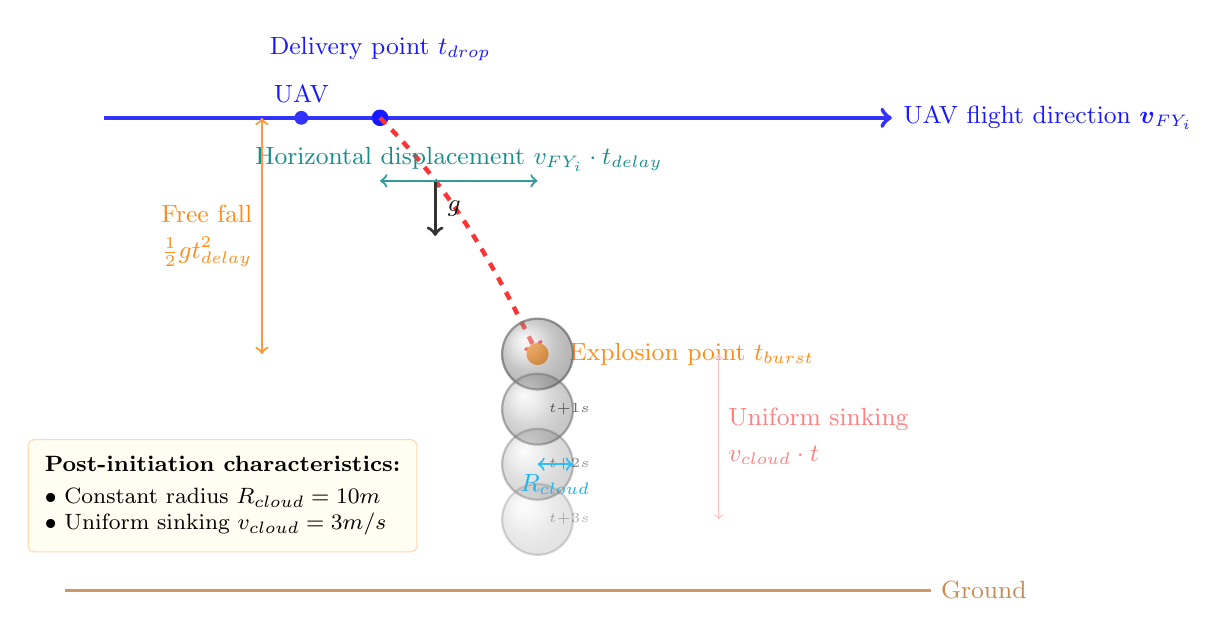
\begin{tikzpicture}[scale=1]
  % UAV trajectory
\draw[blue!80, ultra thick, ->] (0,6) -- (10,6) node[right, blue!90, font=\small] {UAV flight direction $\boldsymbol{v}_{FY_i}$};
\fill[blue!80] (2.5,6) circle (2.5pt) node[above=2pt, blue!90, font=\small] {UAV};

% Delivery point
\fill[blue!90] (3.5,6) circle (3pt);
\node[blue!90, above=3pt, font=\small] at (3.5,6.5) {Delivery point $t_{drop}$};

% Smoke grenade parabolic trajectory (projectile motion)
\draw[red!80, ultra thick, dashed, ->] (3.5,6) .. controls (4.5,5) and (5,4) .. (5.5,3);

% Gravity annotation (moved to the left to avoid blocking the path)
\draw[->, black!80, very thick] (4.2,5.2) -- (4.2,4.5);
\node[black!90, right=1pt, font=\small] at (4.2,4.85) {$g$};

% Explosion point
\fill[orange!90] (5.5,3) circle (4pt);
\node[orange!90, right=8pt, font=\small] at (5.5,3) {Explosion point $t_{burst}$};

% Smoke cloud sinking (same radius, light color)
\def\radius{0.45}
\foreach \t/\y/\opacity/\label in {0/3/0.8/, 1/2.3/0.6/$t{+}1s$, 2/1.6/0.45/$t{+}2s$, 3/0.9/0.3/$t{+}3s$} {
    \draw[gray!, thick, opacity=\opacity] (5.5,\y) circle (\radius);
    \shade[ball color=gray!70, opacity={\opacity*0.5}] (5.5,\y) circle (\radius);
    \ifnum\t>0
        \node[right={1.3*\radius}, black, font=\tiny, opacity=\opacity] at (5.5,\y) {\label};
    \fi
}

% Annotation: Horizontal displacement (moved higher to avoid arrow endpoint)
\draw[<->, teal!80, thick] (3.5,5.2) -- (5.5,5.2);
\node[teal!90, above, font=\small] at (4.5,5.2) {Horizontal displacement $v_{FY_i} \cdot t_{delay}$};

% Annotation: Vertical free fall (left side, light orange)
\draw[<->, orange!80, thick] (2,6) -- (2,3);
\node[orange!90, left, font=\small, align=center] at (2,4.5) {Free fall\\[2pt]$\frac{1}{2}g t_{delay}^2$};

% Annotation: Sinking distance (right side, light pink)
\draw[<->, pink!] (7.8,3) -- (7.8,0.9);
\node[pink!200, right, font=\small, align=left] at (7.8,1.95) {Uniform sinking\\[2pt]$v_{cloud} \cdot t$};

% Ground
\draw[brown!80, very thick] (-0.5,0) -- (10.5,0);
\node[brown!90, right, font=\small] at (10.5,0) {Ground};

% Radius annotation (clearer on the second circle)
\draw[<->, cyan!80, thick] (5.5,1.6) -- (5.5+\radius,1.6);
\node[cyan!90, below, font=\small] at (5.5+\radius/2,1.6) {$R_{cloud}$};
    % Description box (moved to lower left to avoid blocking flight direction)
    \node[draw=orange!30, fill=yellow!5, align=left, font=\footnotesize, inner sep=6pt, rounded corners=2pt] at (1.5,1.2) {
        \textbf{Post-initiation characteristics:}\\[2pt]
        $\bullet$ Constant radius $R_{cloud}=10m$\\
        $\bullet$ Uniform sinking $v_{cloud}=3m/s$
    };
\end{tikzpicture}
\caption{Smoke grenade trajectory and cloud sinking illustration}
\label{fig:smoke_trajectory}
\end{figure}



\subsection{Effective Obstruction Determination Model}
\subsubsection{Geometric Obstruction Conditions}
\paragraph{Problem Background and Simplifying Assumptions}
According to the initial conditions given in the problem, three missiles M1, M2, and M3 are located at (20000,0,2000), (19000,600,2100), and (18000,−600,1900),
UAV FY1 is located at (17800,0,1800), FY2 at (12000,1400,1400), FY3 at (6000,−3000,700),
FY4 at (11000,2000,1800), FY5 at (13000,−2000,1300),
and the true target (a cylinder with base center at $(0,200,0)$, base radius 7 m, and height 10 m) is tens of thousands of meters away from both.
At such a long distance, the geometric size of the target (radius 7 m) is negligible compared to the line of sight length (about 20 km).
Based on the following reasonable assumptions, this paper simplifies the obstruction determination model.
\begin{enumerate}
    \item \textbf{Target Point Simplification}: The true target is simplified to its centroid point $\boldsymbol{P}_T=(0,200,5)$ (base center plus half height 5 m),
    ignoring its geometric size. This simplification is reasonable for long-distance optical/infrared detection and aligns with the small-angle approximation in geometric optics.
    \item \textbf{Missile Field of View Assumption}: The problem does not explicitly limit the missile's field of view. Considering the characteristics of practical inertial-guided missiles,
    it can be assumed that the missile detector's field of view is sufficiently large to cover a reasonable area in the target direction.
    Therefore, only obstruction in the line of sight direction needs to be considered, without considering the field of view boundaries.
    \item \textbf{Line of Sight Segmentation}: The optical detection path of the missile can be abstracted as the line segment $AB$ connecting the missile position $A$ and the target position $B$.
    When the spatial distance between the smoke cloud center and this line segment is less than the smoke radius, the line of sight is effectively obstructed.
\end{enumerate}
Based on the above simplifications, the simplified obstruction schematic relationship is shown in Figure \ref{fig:1}, where the missile line of sight is obstructed if $D \leq R$.
The necessary and sufficient condition for effective obstruction can be expressed as:
\begin{equation}
D(t)\le R_{cloud}
\end{equation}
where $D(t)$ is the \textbf{shortest distance} (point-to-line segment distance) from the smoke cloud center $\boldsymbol{P}_S(t)$ at time $t$ to the line segment $P_{M}(t)P_{T}$ representing the line of sight vector,
$R_{cloud}=10\,\text{m}$ is the effective obstruction radius of the smoke cloud.
Therefore, solving for $D(t)$ is particularly important. Next, we will introduce the method for calculating the distance from a point to a line segment.


\begin{figure}[H]
\centering
\caption{Missile-Smoke Grenade-Target Obstruction Model Schematic}
\label{fig:1}
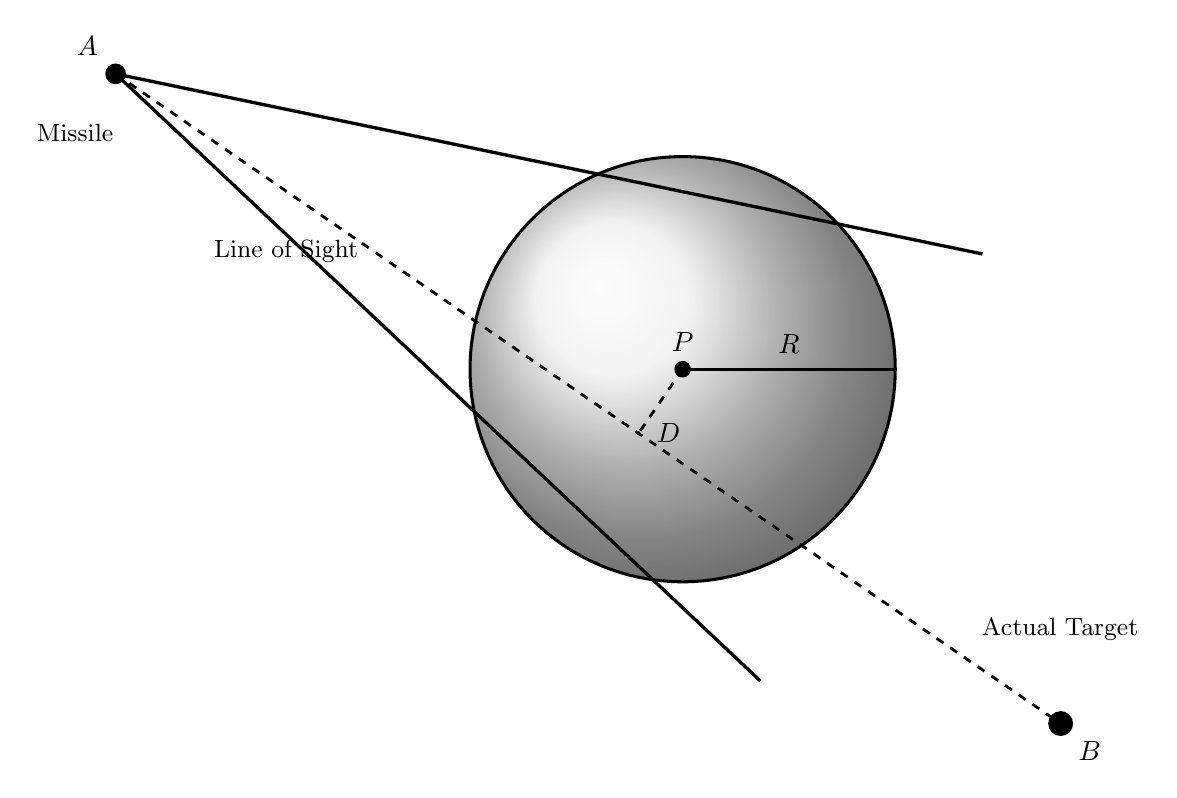
\begin{tikzpicture}[scale=1.5]

% =====================
% Missile Position A (original P1)
% =====================
\coordinate (P1) at (0,5.5);
\fill (P1) circle (2.5pt) node[above left=3pt] {$A$};

% =====================
% The actual target B (the original P2)
% =====================
\coordinate (P2) at (8,0);
\fill (P2) circle (3pt);
\node[below right=3pt] at (P2) {$B$};

% =====================
% Obstructing sphere P (original C)
% =====================
\coordinate (C) at (4.8,3);
\def\radius{1.8}

% Label the distance d at the midpoint of the perpendicular

% =====================
% Calculate the exact tangent lines and tangent points
% =====================
% Distance from A to P
\pgfmathsetmacro{\distPC}{sqrt((4.8-0)^2 + (3-5.5)^2)}
% Direction angle from A to P
\pgfmathsetmacro{\anglePC}{atan2(3-5.5, 4.8-0)}
% Tangent angle with AP (strict calculation)
\pgfmathsetmacro{\tangentAngle}{asin(\radius/\distPC)}

% Positions of the two tangent points (viewed from the sphere center)
\coordinate (T1) at ($(C)+(\anglePC+90-\tangentAngle:\radius)$);
\coordinate (T2) at ($(C)+(\anglePC-90+\tangentAngle:\radius)$);

% =====================
% Draw the sphere (smoke cloud)
% =====================
% Sphere gradient effect
\shade[ball color=gray!14, opacity=0.9] (C) circle (\radius);

% Sphere outline
\draw[line width=1.1pt] (C) circle (\radius);
% Sphere center label
\fill (C) circle (2pt);
\node[above=3pt] at (C) {$P$};

% =====================
% Calculate the foot of the perpendicular from the sphere center P to line A-B and draw the perpendicular
% =====================
% Foot of the perpendicular calculation
\coordinate (FootOfPerpendicular) at ($(P1)!(C)!(P2)$);

% Draw the perpendicular line segment (shortest distance d) - using a prominent color and line style
\draw[dashed, line width=1pt, black] (C) -- (FootOfPerpendicular);

% =====================
% Dashed line from A to B (obstructed direct line of sight)
% =====================
\draw[dashed, line width=1pt] (P1) -- (P2);

% Draw a small mark at the foot of the perpendicular
\fill[black] (FootOfPerpendicular) circle (0.5pt);

% Radius annotation (draw the radius line)
\draw[line width=1pt] (C) -- ($(C)+(\radius,0)$);
\node[above=2pt] at ($(C)+(\radius/2,0)$) {$R$};
\node[right=3pt, font=\normalsize, black] at ($(C)!1!(FootOfPerpendicular)$) {$D$};

% =====================
% A's observation tangent lines (only up to the tangent points)
% =====================
\draw[line width=1.2pt] (P1) -- ($(P1)!1.2!(T1)$);
\draw[line width=1.2pt] (P1) -- ($(P1)!1.2!(T2)$);

% =====================
% Annotation Explanation
% =====================
\node[text width=2cm, font=\small, align=left] at (0,5) {Missile};
\node[text width=2cm, font=\small, align=left] at (1.5,4) {Line of Sight};
\node[text width=2cm, font=\small, align=left] at (8,0.8) {Actual Target};
\end{tikzpicture}
\end{figure}
\subsubsection{Point-to-Segment Distance Algorithm}
Let the missile position be point A, the actual target position be point B, and the smoke grenade center be point P. The vector $\overrightarrow{AB}=B-A$, and the vector $\overrightarrow{AP}=P-A$. The projection coefficient r is calculated as:
\begin{equation}
r=\frac{\overrightarrow{AP}\cdot\overrightarrow{AB}}{\|\overrightarrow{AB}\|^2}
\end{equation}
The distance is discussed in three cases, as shown in Figure \ref{fig:distance_cases}:
\begin{equation}D(t)=\begin{cases}
\|\overrightarrow{AP}\| & \text{if } r \leq 0 \text{ (behind the missile)}\\
\|P-B\| & \text{if } r \geq 1 \text{ (behind the target)}\\
\frac{\|\overrightarrow{AP}\times\overrightarrow{AB}\|}{\|\overrightarrow{AB}\|} & \text{if } 0<r<1 \text{ (projection within the segment)}
\end{cases}\end{equation}
\begin{figure}[H]
\centering
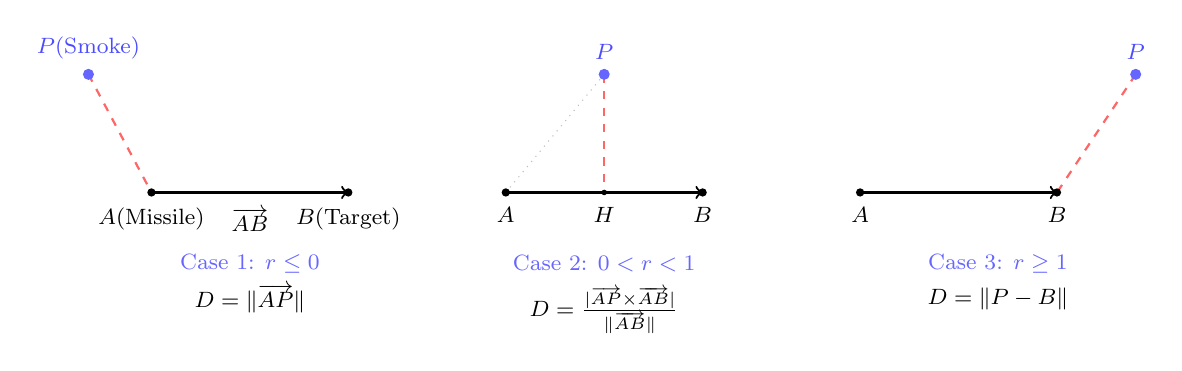
\begin{tikzpicture}[scale=1.0]
    % Case 1: r <= 0 (behind the missile)
    \begin{scope}[shift={(0,0)}]
        \coordinate (A) at (0,0);
        \coordinate (B) at (2.5,0);
        \coordinate (P) at (-0.8,1.5);
        
        \draw[thick,->] (A) -- (B) node[midway,below=2pt,font=\footnotesize] {$\overrightarrow{AB}$};
        \draw[dashed,red!60,thick] (P) -- (A);
        \fill (A) circle (1.5pt) node[below=2pt,font=\footnotesize] {$A$(Missile)};
        \fill (B) circle (1.5pt) node[below=2pt,font=\footnotesize] {$B$(Target)};
        \fill[blue!60] (P) circle (2pt) node[above=2pt,font=\footnotesize,blue!70] {$P$(Smoke)};
        
        \node[blue!60,font=\footnotesize] at (1.25,-0.9) {Case 1: $r \leq 0$};
        \node[font=\footnotesize] at (1.25,-1.35) {$D = \|\overrightarrow{AP}\|$};
    \end{scope}
    
    % Case 2: 0 < r < 1 (projection within the segment)
    \begin{scope}[shift={(4.5,0)}]
        \coordinate (A) at (0,0);
        \coordinate (B) at (2.5,0);
        \coordinate (P) at (1.25,1.5);
        \coordinate (H) at (1.25,0);
        
        \draw[thick,->] (A) -- (B);
        \draw[dashed,red!60,thick] (P) -- (H);
        \draw[dotted,gray!50] (A) -- (P);
        \fill (A) circle (1.5pt) node[below=2pt,font=\footnotesize] {$A$};
        \fill (B) circle (1.5pt) node[below=2pt,font=\footnotesize] {$B$};
        \fill[blue!60] (P) circle (2pt) node[above=2pt,font=\footnotesize,blue!70] {$P$};
        \fill (H) circle (1pt) node[below=2pt,font=\footnotesize] {$H$};
        
        \node[blue!60,font=\footnotesize] at (1.25,-0.9) {Case 2: $0 < r < 1$};
        \node[font=\footnotesize,align=center] at (1.25,-1.5) {$D = \frac{|\overrightarrow{AP} \times \overrightarrow{AB}|}{\|\overrightarrow{AB}\|}$};
    \end{scope}
    
    % Case 3: r >= 1 (behind the target)
    \begin{scope}[shift={(9,0)}]
        \coordinate (A) at (0,0);
        \coordinate (B) at (2.5,0);
        \coordinate (P) at (3.5,1.5);
        
        \draw[thick,->] (A) -- (B);
        \draw[dashed,red!60,thick] (P) -- (B);
        \fill (A) circle (1.5pt) node[below=2pt,font=\footnotesize] {$A$};
        \fill (B) circle (1.5pt) node[below=2pt,font=\footnotesize] {$B$};
        \fill[blue!60] (P) circle (2pt) node[above=2pt,font=\footnotesize,blue!70] {$P$};
        
        \node[blue!60,font=\footnotesize] at (1.75,-0.9) {Case 3: $r \geq 1$};
        \node[font=\footnotesize] at (1.75,-1.35) {$D = \|P - B\|$};
    \end{scope}
\end{tikzpicture}
\caption{Three cases of point-to-segment distance calculation}
\label{fig:distance_cases}
\end{figure}
\subsection{Shading Time Model}
\subsubsection{Shading Indicator Function}
To quantitatively describe the shielding effect of the smoke cloud layer on missiles, the \textbf{shielding indicator function} $I_j(t)$ is introduced,
which is used to represent whether the $j$-th missile is effectively shielded at time $t$.
The function is defined as:
\begin{equation}
I_j(t)=\begin{cases}1,&\text{if } D_{k,j}(t)\le R_{cloud} \text{ and } t\geq t_{burst,k}\\0,&\text{otherwise}\end{cases}
\end{equation}
Here, $D_{k,j}(t)$ represents the point-to-line segment distance between the $k$th smoke grenade and the $j$th missile at time $t$. $R_{cloud} = 10\,\text{m}$: the effective shielding radius of the smoke cloud. $t_{burst,k}$ is the detonation time of the $k$th smoke grenade.
This indicator function has the following physical meaning:
\begin{enumerate}
    \item When $t < t_{burst,k}$, the smoke grenade has not yet detonated, so $I_j(t)=0$ (no shielding).
    \item When $t \geq t_{burst,k}$ and $D_{k,j}(t)\le R_{cloud}$, the smoke cloud effectively blocks the line of sight, so $I_j(t)=1$ (effective shielding).
    \item When $D_{k,j}(t) > R_{cloud}$, the smoke cloud is too far from the line of sight, so $I_j(t)=0$ (shielding ineffective).
\end{enumerate}
\subsubsection{Total Effective Shading Duration}
For a single missile $j$, the total effective shading duration during the entire flight process $[0,T_{end}]$ is defined as the time integral of the indicator function.
\begin{equation}
T_j=\int_0^{T_{end}}{I_j(t) \,dt}
\end{equation}
Here, $T_{end}$ is the missile flight termination time. Through this integral, we can calculate the cumulative time during which the missile is effectively shaded by the smoke cloud throughout its flight.
In scenarios involving multiple missiles ($M_1,M_2,\ldots,M_m$) cooperating in interception,
the overall system optimization objective is defined as the sum of the shading durations of all missiles:
\begin{equation}
\max\, T_{cover} = \sum_{j=1}^{m} T_j
\end{equation}
This objective function reflects the tactical requirement of "maximizing overall protection effectiveness."
\subsubsection{Time Discretization Strategy}
Due to the continuous time-varying motion of multiple entities such as missiles and smoke clouds in the system,
and the shielding determination conditions involving complex geometric relationships and nonlinear logic,
it is not possible to directly solve the shading time integral $\int_0^{T_{end}} I_j(t) dt$ analytically.
Therefore, this paper adopts a time discretization method, as shown in Figure \ref{fig:time_discretization}, dividing the continuous time axis into equally spaced discrete time points:
\begin{equation}
t_k = k \Delta t, \quad k = 0, 1, 2, \ldots, N
\end{equation}
where $\Delta t$ is the time step size, and $N = \lfloor T_{end}/\Delta t \rfloor$.
At each discrete time point $t_k$, first, based on the kinematic equations, update the missile position $\boldsymbol{P}_{M_j}(t_k)$ and the center position of the smoke cloud $\boldsymbol{P}_{S,k}(t_k)$.
Then, calculate the distance from the point to the line segment $D_{k,j}(t_k)$.
Next, according to the shielding determination conditions, determine the shielding state $I_j(t_k) \in \{0, 1\}$.
Finally, the effective shielding duration can be approximated by the \textbf{Riemann sum}:
\begin{equation}
T_{cover} \approx \sum_{k=0}^{N} I(t_k) \cdot \Delta t
\end{equation}
This formula essentially represents the numerical calculation of a definite integral. As $\Delta t \to 0$, the discrete sum converges to the exact value of the continuous integral.
The choice of time step size must balance computational accuracy and efficiency:
\begin{itemize}
    \item \textbf{Coarse scanning phase} (initial search): $\Delta t = 0.1s$, quickly locating potential shading intervals
    \item \textbf{Fine calculation phase} (optimization solving): $\Delta t = 0.01s$ or $0.001s$, ensuring accuracy
\end{itemize}
This method is not only suitable for single-target single-missile scenarios,
but also efficiently handles overlapping time windows and shading unions in multi-UAV multi-missile cooperative problems.
\begin{figure}[H]
\centering
\caption{Time Discretization and Accumulation of Shading Duration}
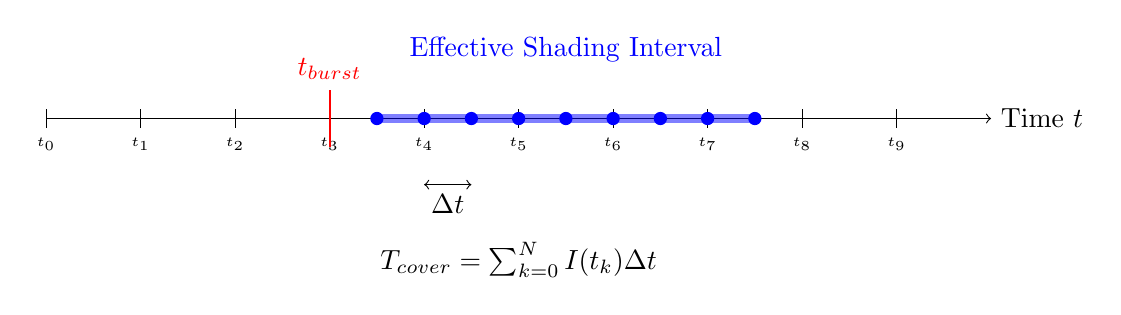
\begin{tikzpicture}[scale=1.2]
    % Time axis
    \draw[->] (0,0) -- (10,0) node[right] {Time $t$};
    
    % Time point markers
    \foreach \x in {0,1,2,...,9} {
        \draw (\x,0.1) -- (\x,-0.1);
        \node[below] at (\x,-0.1) {\tiny $t_{\x}$};
    }
    
    % Burst time
    \draw[red, thick] (3,-0.3) -- (3,0.3) node[above] {$t_{burst}$};
    
    % Effective shielding interval
    \draw[blue, line width=3pt, opacity=0.5] (3.5,0) -- (7.5,0);
    \node[above, blue] at (5.5,0.5) {Effective Shading Interval};
    
    % Discrete point determination
    \foreach \x in {3.5,4,4.5,5,5.5,6,6.5,7,7.5} {
        \fill[blue] (\x,0) circle (2pt);
    }
    
    % Step size annotation
    \draw[<->] (4,-0.7) -- (4.5,-0.7) node[midway, below] {$\Delta t$};
    
    % Integration illustration
    \node[align=center] at (5,-1.5) {$T_{cover} = \sum_{k=0}^{N} I(t_k) \Delta t$};
\end{tikzpicture}

\label{fig:time_discretization}
\end{figure}






\section{Model Solution}

\subsection{Problem 1 Solution: Fixed Parameters}
Problem 1 focuses on a specific scenario where all parameters (smoke grenade deployment time, detonation time) are given, and the goal is to calculate the effective shading time of a single smoke grenade against a single missile.
We need to use the position functions of each object combined with the effective shading criteria to obtain the effective shading time.
The problem provides the flight strategy of UAV FY1 (speed, heading) and the bomb deployment strategy (deployment time, detonation delay),
The core task of this question is \textbf{simulation verification} of the effectiveness of the known strategy.
Unlike the subsequent optimization problems (Problems 2 to 5), Problem 1 does not require searching for the optimal solution,
but is based on deterministic inputs for numerical simulation.
Therefore, a \textbf{time discretization simulation method} can be directly used to solve it.
\paragraph{Overview of Solution Steps}
\begin{enumerate}
    \item \textbf{Parameter Substitution}: Substitute all given physical parameters into the kinematic equations
    \item \textbf{Trajectory Calculation}: Calculate the detonation position of the smoke grenade and the time-varying positions of all entities
    \item \textbf{Shading Determination}: Check at each time step whether the smoke cloud effectively shades the missile's line of sight
    \item \textbf{Duration Statistics}: Accumulate the time intervals that meet the shading conditions to obtain the total shading duration
\end{enumerate}
\subsubsection{Parameter Substitution and Scenario Setup}
According to the problem conditions, the initial parameters of each entity are as follows:
\paragraph{UAV FY1 Parameters}
\begin{itemize}
    \item Initial Position: $\mathbf{P}_{FY_1}(0)=(17800,\,0,\,1800)\,\text{m}$
    \item Flight Speed: $v_{FY_1}=120\,\text{m/s}$
    \item Flight Heading: Directed towards the false target $\boldsymbol{P}_O=(0,0,0)$,
    i.e., velocity vector $\boldsymbol{v}_{FY_1}=(-120,0,0)\,\text{m/s}$
\end{itemize}

\paragraph{Missile M1 Parameters}
\begin{itemize}
    \item Initial Position: $\mathbf{P}_{M_1}(0)=(20000,\,0,\,2000)\,\text{m}$
    \item Flight Speed: $V_m=300\,\text{m/s}$ (directed towards the false target)
    \item Flight Direction: Unit vector $\mathbf{n}_{M_1}=\frac{\boldsymbol{P}_O-\mathbf{P}_{M_1}(0)}{\|\boldsymbol{P}_O-\mathbf{P}_{M_1}(0)\|}$
\end{itemize}

\paragraph{Smoke Grenade Deployment Strategy}
\begin{itemize}
    \item Deployment Time: $t_{drop}=1.5\,\text{s}$ (deployed 1.5 seconds after receiving the task)
    \item Detonation Delay: $t_{delay}=3.6\,\text{s}$ (detonates 3.6 seconds after deployment)
    \item Detonation Time: $t_{burst}=t_{drop}+t_{delay}=5.1\,\text{s}$
\end{itemize}

\paragraph{Smoke Cloud Physical Parameters}
\begin{itemize}
    \item Effective Radius: $R_{cloud}=10\,\text{m}$
    \item Sinking Speed: $v_{cloud}=3\,\text{m/s}$
    \item Effective Duration: Maintains shading capability for 20 seconds after detonation
\end{itemize}
\subsubsection{Trajectory Calculation}
Based on the motion models established earlier, the spatial positions of all entities in the system vary with time.
The UAV's position at the deployment time is
$
\mathbf{P}_{FY_1}
=
\mathbf{P}_{FY_1}(t_{drop}).
$,The detonation time of the smoke grenade is
\begin{equation}
t_{burst}=t_{drop}+t_{delay},
\end{equation}
then its detonation position is
\begin{equation}
\mathbf{P}_{burst}
=
\mathbf{P}_{FY_1}(t_{drop})
+
\boldsymbol{v}_{FY_1}t_{delay}
-
\left(0,\,0,\,\tfrac{1}{2}gt_{delay}^2\right).
\end{equation}
After detonation, the center of the smoke cloud sinks vertically at a constant speed. Its position at any time $t$ is
\begin{equation}
\mathbf{P}_{S}(t)
=
\mathbf{P}_{burst}
-
\left(0,\,0,\,v_{cloud}(t-t_{burst})\right),
\quad t\ge t_{burst}.
\end{equation}
The position of missile M1 at any time $t$ is
\begin{equation}
\mathbf{P}_{M}(t)
=
\mathbf{P}_{M}(0)
+
V_M\mathbf{n}_M t,
\end{equation}
where $\mathbf{n}_M$ is the unit direction vector of the missile pointing towards the false target.

\subsubsection{Effective Shading Duration Calculation}
To calculate the effective shading duration, the time interval $[0,T_{end}]$ is discretized.
The time step is taken as $\Delta t=0.05\,\text{s}$, and the end time $T_{end}$ is the time when the missile reaches the false target.
Discrete time points are defined as:
\begin{equation}
t_k=k\Delta t,\quad k=0,1,\ldots,N,\quad N=\lfloor T_{end}/\Delta t\rfloor
\end{equation}

\paragraph{Step-by-Step Shading Determination}
At each discrete time $t_k$, the following determination process is executed:
\begin{enumerate}
    \item \textbf{Time Window Check}: If $t_k < t_{burst}$ or $t_k > t_{burst}+20$,
    the smoke grenade has not detonated or has expired, so $I(t_k)=0$
    \item \textbf{Spatial Position Update}: Calculate $\mathbf{P}_{M_1}(t_k)$, $\mathbf{P}_S(t_k)$, and the true target position $\mathbf{P}_T=(0,200,5)$
    \item \textbf{Distance Calculation}: Calculate the shortest distance $D(t_k)$ from the center of the smoke cloud to the line connecting the "missile-target" (point-to-line segment distance algorithm)
    \item \textbf{Obstruction Detection}: If $D(t_k) \le R_{cloud} = 10\,\text{m}$, then $I(t_k) = 1$; otherwise, $I(t_k) = 0$
\end{enumerate}

The shielding indicator function is defined as:
\begin{equation}
I(t_k)=
\begin{cases}
1, & D(t_k)\le R_{cloud}\ \text{and}\ t_k\in[t_{burst},t_{burst}+20],\\
0, & \text{otherwise}.
\end{cases}
\end{equation}

\paragraph{Total Duration Statistics}
By summing all time points that satisfy the shading condition, the total effective shading duration is obtained:
\begin{equation}
T_{cover}=\sum_{k=0}^{N} I(t_k)\cdot\Delta t
\end{equation}

\subsubsection{Model Summary}


Comprehensive analysis above, the solution model for Problem 1 can be summarized as:
\begin{equation}
\left\{
\begin{aligned}
& \text{\textbf{Input Parameters}}:\quad \mathbf{P}_{FY_1}(0),\,v_{FY_1},\,t_{drop},\,t_{delay},\,\mathbf{P}_{M_1}(0),\,V_m \\
& \text{\textbf{Missile Motion}}:\quad \mathbf{P}_{M_1}(t)=\mathbf{P}_{M_1}(0)+V_m\mathbf{n}_{M_1}\cdot t \\
& \text{\textbf{Drone Motion}}:\quad \mathbf{P}_{FY_1}(t)=\mathbf{P}_{FY_1}(0)+\boldsymbol{v}_{FY_1}\cdot t \\
& \text{\textbf{Burst Position}}:\quad \mathbf{P}_{burst}=\mathbf{P}_{FY_1}(t_{drop})+\boldsymbol{v}_{FY_1}\cdot t_{delay}-(0,0,\tfrac{1}{2}gt_{delay}^2) \\
& \text{\textbf{Cloud Motion}}:\quad \mathbf{P}_{S}(t)=\mathbf{P}_{burst}-(0,0,v_{cloud}(t-t_{burst})),\quad t\ge t_{burst} \\
& \text{\textbf{Distance Calculation}}:\quad D(t)=\begin{cases}
\|\mathbf{P}_S(t)-\mathbf{P}_{M_1}(t)\| & \text{if } r \leq 0\\
\|\mathbf{P}_T-\mathbf{P}_S(t)\| & \text{if } r \geq 1 \\
\frac{\|(\mathbf{P}_S(t)-\mathbf{P}_{M_1}(t))\times(\mathbf{P}_T-\mathbf{P}_{M_1}(t))\|}{\|\mathbf{P}_T-\mathbf{P}_{M_1}(t)\|} & \text{if } 0<r<1 
\end{cases} \\
& \text{\textbf{Obstruction Detection}}:\quad I(t)=\begin{cases}1,&D(t)\le R_{cloud}\ \text{and}\  t_{burst} \le t \le t_{burst}+20\\0,&\text{otherwise}\end{cases} \\
& \text{\textbf{Output}}:\quad T_{cover}=\int_0^{T_{end}}{I(t)\,dt}\approx\sum_{k=0}^{N}I(t_k)\cdot\Delta t
\end{aligned}
\right.
\end{equation}

where the projection coefficient is defined as $r=\frac{(\mathbf{P}_S(t)-\mathbf{P}_{M_1}(t))\cdot(\mathbf{P}_T-\mathbf{P}_{M_1}(t))}{\|\mathbf{P}_T-\mathbf{P}_{M_1}(t)\|^2}$.


\subsubsection{Solution Results:} After calculation, the results are shown in Figure \ref{fig:2}, clearly demonstrating the effective duration of the smoke cloud. The smoke grenade burst time is $t=5.10 s$,
the initial burst coordinates are $(17188.00,0.00,1736.50)$, the effective shading duration is $8.1-9.5s$, with a total duration of $1.4s$.
    \begin{figure}[H]
        \centering
        \includegraphics[width=0.8\textwidth]{images/pro1.png}
        \caption{Problem 1 Results}
        \label{fig:2}
    \end{figure}
\subsection{Problem 2 Solution: Single Drone Single Grenade Optimization}
Problem 2 is a generalization and extension of Problem 1. Unlike Problem 1, which involves simulation verification with given parameters, Problem 2 requires optimizing the flight strategy and grenade dropping strategy of drone FY1 under \textbf{adjustable parameters} to maximize the effective shading time of a single smoke grenade against missile M1.
The core challenge of this problem is that the number of decision variables increases from 0 (all given in Problem 1) to 4, and the objective function $T_{cover}(X)$ is highly nonlinear and non-convex, making it impossible to solve analytically.
Therefore, a \textbf{nonlinear programming model} needs to be established, and intelligent optimization algorithms should be used for numerical solutions.
\subsubsection{Decision Variables}
According to the problem requirements, once the drone receives the task, its speed and heading are determined and no longer adjusted.
Therefore, when making task decisions, we need to decide the following four variables:
As shown in Table \ref{tab:1}
\begin{table}[H]
\centering
\caption{Description of Decision Variables for Problem 2}
\label{tab:1}
\begin{tabularx}{\linewidth}{>{\bfseries}lXc}
\toprule
Variable & Physical Meaning & Range \\
\midrule
$v_{FY_1}$ & Drone flight speed & $[70,140]\,\text{m/s}$ \\
$\alpha$ & Drone heading angle (relative to $x$-axis) & $[0,2\pi)\,\text{rad}$ \\
$t_{drop}$ & Smoke grenade drop time & $[0,12]\,\text{s}$ \\
$t_{delay}$ & Smoke grenade burst delay & $[1,8]\,\text{s}$ \\
\bottomrule
\end{tabularx}
\end{table}

Define the decision vector as:
\begin{equation}
X=[v_{FY_1},\,\alpha,\,t_{drop},\,t_{delay}]^T\in\mathbb{R}^4
\end{equation}

These four variables are not independent but are coupled through physical constraints:
\begin{itemize}
    \item \textbf{Speed-Heading Coupling}: $v_{FY_1}$ and $\alpha$ jointly determine the drone's flight trajectory,
    which in turn affects the smoke grenade drop position $\boldsymbol{P}_{drop}$
    \item \textbf{Time-Space Coupling}: $t_{drop}$ determines the drop position, and $t_{delay}$ determines the burst position,
    both of which jointly affect the relative position between the smoke cloud and the missile's line of sight
    \item \textbf{Altitude Constraint Coupling}: A large $t_{delay}$ may cause the smoke grenade to burst after hitting the ground (violating physical constraints),
    so the feasible domain of $t_{delay}$ is indirectly constrained by $v_{FY_1}$, $\alpha$, and $t_{drop}$
\end{itemize}

\subsubsection{State Equations}
Based on the kinematic model established in Problem 1, the decision variables $X$ are parameterized and embedded into the state equations\\
Convert scalar speed $v_{FY_1}$ and heading angle $\alpha$ into a three-dimensional velocity vector:
\begin{equation}
\boldsymbol{v}_{FY_1}(v_{FY_1},\alpha)=[v_{FY_1}\cos\alpha,\,v_{FY_1}\sin\alpha,\,0]^T
\end{equation}
Drop point position (dependent on $v_{FY_1}$, $\alpha$, $t_{drop}$)
\begin{equation}
\boldsymbol{P}_{drop}(X)=\boldsymbol{P}_{FY_1}(0)+\boldsymbol{v}_{FY_1}(v_{FY_1},\alpha)\cdot t_{drop}
\end{equation}
Burst point position (dependent on all four decision variables):
\begin{equation}
\boldsymbol{P}_{burst}(X)=\boldsymbol{P}_{drop}(X)+\boldsymbol{v}_{FY_1}(v_{FY_1},\alpha)\cdot t_{delay}+[0,0,-\tfrac{1}{2}gt_{delay}^2]^T
\end{equation}
Smoke cloud center trajectory ($t\geq t_{burst}$):
\begin{equation}
\boldsymbol{P}_S(t;X)=\boldsymbol{P}_{burst}(X)-[0,0,v_{cloud}(t-t_{burst})]^T
\end{equation}
\subsubsection{Objective Function}
The objective is to maximize the effective coverage duration, using the coverage indicator function defined in Problem 1 to derive the objective function:
\begin{equation}
maxJ\left(X\right)=T_{cover}={\int}_0^{T_{end}}I\left(t;X\right)dt
\end{equation}
Among them, the masking indicator function depends on the decision variable $X$:
\begin{equation}
I(t;X)=\begin{cases}
1, & D(t;X)\le R_{cloud}\text{ and }t\geq t_{burst}(X)\\
0, & \text{otherwise}
\end{cases}
\end{equation}
$D(t;X)$ is the distance from the smoke cloud center $\boldsymbol{P}_S(t;X)$ to the missile's line of sight (point-to-line segment distance).
\subsubsection{Constraints}
Based on the problem requirements and analysis of the model's velocity characteristics, the constraints are as follows:\\
\quad Speed constraint: After receiving the mission, the drone instantaneously adjusts its flight direction, then flies at a constant altitude with a uniform linear speed between 70 and 140 m/s
\begin{equation}
70\le v_{FY_1}\le140
\end{equation}
Time constraint: The upper limit of the drop time is 12 seconds considering the missile's flight speed; dropping too late may miss the interception opportunity.
\begin{equation}
0\le t_{drop}\le12,1\le t_{delay}\le8
\end{equation}  
Altitude constraint: The smoke grenade must burst in the air, so the burst point's altitude must be greater than zero
\begin{equation}
z_{burst}\left(X\right)>0
\end{equation}
\subsubsection{Model Summary}
Based on the above analysis, the complete optimization model for Problem 2 can be expressed as:
\begin{equation}
\left\{
\begin{aligned}
& \text{Decision variables:}\quad X=[v_{FY_1},\alpha,t_{drop},t_{delay}]^T \\
& \text{Objective function:}\quad \max\ T_{cover}(X)=\int_0^{T_{end}}I(t;X)dt \\
& \text{State equations:}\quad \begin{cases}
\boldsymbol{v}_{FY_1}=v_{FY_1}[\cos\alpha,\sin\alpha,0]^T\\
\boldsymbol{P}_{drop}=\boldsymbol{P}_{FY_1}(0)+\boldsymbol{v}_{FY_1}\cdot t_{drop}\\
\boldsymbol{P}_{burst}=\boldsymbol{P}_{drop}+\boldsymbol{v}_{FY_1}\cdot t_{delay}+[0,0,-\frac{1}{2}gt_{delay}^2]^T\\
\boldsymbol{P}_S(t)=\boldsymbol{P}_{burst}-[0,0,v_{cloud}(t-t_{burst})]^T
\end{cases}\\
& \text{Coverage determination:}\quad I(t;X)=\begin{cases}
1, & D(t)\le R_{cloud}\text{ and } t_{burst}\le t \le t_{burst}+20\\
0, & \text{otherwise}
\end{cases}\\
& \text{Constraints:}\quad \begin{cases}
70\le v_{FY_1}\le 140\\
0\le t_{drop}\le 12,\quad 1\le t_{delay}\le 8\\
z_{burst}(X)>0
\end{cases}
\end{aligned}
\right.
\end{equation}


\subsubsection{Solution Algorithm}
Due to the complex geometric motion and piecewise logic involved in the objective function, it exhibits high nonlinearity and non-convexity, and the decision variables have higher degrees of freedom compared to typical single-variable optimization problems.
Therefore, to solve such problems, this problem adopts a two-level optimization strategy, with grid search in the outer loop and particle swarm optimization (PSO) in the inner loop. This reduces the optimization problem dimension from 4 to 3, lowering the search difficulty and reducing the probability of the problem falling into local optima.\\
\textbf{Outer loop:}


We use the \textbf{grid search method}, first discretizing the speed $v_{FY_1}$ in the interval $[70,140]$ with a step size of $\Delta v=0.5\,\text{m/s}$
\begin{equation}
v_{FY_1}\in\{70.0,\,70.5,\,71.0,\,\ldots,\,139.5,\,140.0\}
\end{equation}
Then, for each discrete speed value, the inner PSO algorithm is called to solve the subproblem
\begin{equation}
\max_{(\alpha,t_{drop},t_{delay})}\,T_{cover}(v_{FY_1},\alpha,t_{drop},t_{delay})
\end{equation}
Record the optimal solution $(\alpha^*,t_{drop}^*,t_{delay}^*)$ and its objective function value corresponding to each $v_{FY_1}$,
and finally select the global optimum.\\
\textbf{Inner loop:}


We use the particle swarm optimization algorithm (PSO). First, we perform
\textbf{particle encoding}, representing the position of the $i$-th particle as $x_i=[\alpha_i,t_{drop,i},t_{delay,i}]$, and its velocity as $v_i$; thus, each particle represents a candidate solution $x_i$,
Then we proceed with \textbf{parameter setting}, setting the population size to $N$ to 30, the maximum number of iterations $G_{max}$ to 50 times, the inertia weight $w=$ to 0.6 to balance global and local search, and the learning factors $c_1=c_2$ to 1.5 to balance individual cognition and social learning.
Meanwhile, the \textbf{velocity and position update formulas for particles} are
\begin{align}
v_i^{k+1} &= w\cdot v_i^k+c_1r_1\odot(p_{best,i}-x_i^k)+c_2r_2\odot(g_{best}-x_i^k) \\
x_i^{k+1} &= x_i^k+v_i^{k+1}
\end{align}
Among them, $r_1, r_2 \sim \text{Uniform}(0,1)$ are random numbers, $\odot$ represents element-wise multiplication, $p_{best,i}$ is the historical best position of particle $i$, and $g_{best}$ is the global best position.
In each iteration, the algorithm adjusts the particle positions using the above update formulas and evaluates the quality of each particle solution through the fitness function,
thereby updating the individual historical best $p_{best,i}$ and the global best $g_{best}$.
\textbf{Fitness function} $F\left(x\right)$ is defined as the negative of the coverage time (converted to a minimization problem):
\begin{equation}
F\left(x\right)=-T_{cover}\left(x\right)
\end{equation}
The algorithm continues to iterate until the maximum number of iterations or convergence criteria are met, finally outputting the global optimal solution $g_{best}$ and the corresponding maximum coverage time.
\subsubsection{Solution Results}
Based on the MATLAB-implemented two-level optimization algorithm (code in the appendix), the optimal deployment strategy is as follows:\\
The UAV flies at a heading angle of 176.91°, a speed of 72 m/s, drops at 0 s, detonates after 2.4991 s, with an effective coverage time of 4.738 s, as shown in Figure \ref{fig:3}.
Compared to the 1.4 s in Problem 1, this is an improvement of $238\%$.




\begin{figure}[H]
    \centering
    \includegraphics[width=0.8\textwidth]{images/pro2.png}
    \caption{the results of Problem 2}
    \label{fig:3}
\end{figure}
\subsection{Problem 3 Solution: Multi-Projectile Coordination Strategy}
In this problem, the UAV FY1 needs to continuously deploy 3 smoke grenades to interfere with missile M1.
Unlike deploying a single smoke grenade, the deployment strategy for three smoke grenades involves temporal coordination, with the core issue being the optimization of multiple parameters to maximize the smoke grenade coverage time.

\subsubsection{Decision Variables}
According to the problem requirements, once the UAV receives the mission, its speed and heading are fixed and no longer adjusted. Therefore, in mission decision-making, we need to decide the following eight variables \ref{tab:2}:
Flight speed $v_{FY_1}$
, flight heading angle $\alpha$
, drop times \quad $t_{drop,i} \quad (i \in\{1,2,3\})$
, delayed detonation times \quad $t_{delay,i} \quad, (i \in\{1,2,3\})$
, thereby defining the decision vector $\mathbf{X}$:
\begin{equation}
\mathbf{X}=[v_{FY_1},\,\alpha,\,t_{drop,1},\,t_{drop,2},\,t_{drop,3},\,t_{delay,1},\,t_{delay,2},\,t_{delay,3}]^T\in\mathbb{R}^8
\end{equation}
\begin{table}[H]
\centering
\caption{Decision Variables and Constraints for Problem 3}
\label{tab:2}
\begin{tabularx}{\linewidth}{lXc}
\toprule
\textbf{Variable Type} & \textbf{Specific Variable} & \textbf{Constraint Range} \\
\midrule
\multirow{2}{*}{Global Flight Parameters} & $v_{FY_1}$ & $[70,140]\,\text{m/s}$ \\
& $\alpha$ & $[0,2\pi)\,\text{rad}$ \\
\multirow{3}{*}{Drop Times} & $t_{drop,1}$ & $[0,12]\,\text{s}$ \\
& $t_{drop,2}$ & $[t_{drop,1}+1,12]\,\text{s}$ \\
& $t_{drop,3}$ & $[t_{drop,2}+1,12]\,\text{s}$ \\
\multirow{3}{*}{Delayed Detonation Times} & $t_{delay,1}$ & $[1,8]\,\text{s}$ \\
& $t_{delay,2}$ & $[1,8]\,\text{s}$ \\
& $t_{delay,3}$ & $[1,8]\,\text{s}$ \\
\bottomrule
\end{tabularx}
\end{table}



\subsubsection{Multi-Projectile Motion State Equations}
Based on the single projectile motion model established in Problem 1, it is extended to a multi-projectile scenario.
The motion state of the $k$-th smoke grenade is described by the following equations:
\\
1.	Drop Point Coordinates:
\begin{equation}
    P_{drop,k}(\mathbf{X})=B_0+\boldsymbol{v}_{FY_1}(v_{FY_1},\alpha)\cdot t_{drop,k}
\end{equation}
2.	Burst Point Coordinates:
\begin{equation}
P_{burst,k}(\mathbf{X})=P_{drop,k}(\mathbf{X})+\boldsymbol{v}_{FY_1}(v_{FY_1},\alpha)\cdot t_{delay,k}+\left[0,0,-\frac{1}{2}gt_{delay,k}^2\right]^T
\end{equation}
3.	Smoke Cloud Center Trajectory:
After the burst time $\ t_{burst,k}=t_{drop,k}+t_{delay,k} $, the position of the $k$-th cloud center is
\begin{equation}
    P_{S,k}(t)=P_{burst,k}-[0,0,v_{cloud}\cdot(t-t_{burst,k})]^T \quad ,\quad t\in[t_{burst,k},t_{burst,k}+20]
\end{equation} 
This time window $[t_{burst,k},t_{burst,k}+20]$ represents the effective duration of the $k$-th smoke grenade being 20 seconds.
\subsubsection{Objective Function}


Define the coverage state of the $k$-th smoke grenade at time $t$ as:
\begin{equation}
I_k(t;\mathbf{X})=\begin{cases}
1, & D_k(t) \leq R_{cloud}\text{ and }t \in [t_{burst,k}, t_{burst,k}+20] \\
0, & \text{otherwise}
\end{cases}
\end{equation}
Here, $D_k(t)$ is the shortest distance from the center of the $k$-th smoke cloud to the line of sight between missile $M_1$ and target $P_T$.
\textbf{System Total Coverage State (Logical OR)}
Since the three smoke clouds may exist simultaneously, the system coverage state at time $t$ is defined as the \textbf{logical OR}:
\begin{equation}
I_{total}(t;\mathbf{X}) = \bigvee_{k=1}^{3}I_{k}(t;\mathbf{X}) 
\end{equation}
Here, $\bigvee_{k=1}^{3}$ is the logical OR operator.
The physical meaning of this definition is: as long as \textbf{at least one} smoke grenade is effectively covering,
the missile is considered to be in a covered state ($I_{total}=1$).
The final optimization objective is to maximize the total effective coverage duration $T_{cover}$ defined as the time integral of the indicator function:
\begin{equation}
\max\,J(\mathbf{X})=T_{cover}(\mathbf{X})=\int_{0}^{T_{end}}I_{total}(t;\mathbf{X})\,dt
\end{equation}
This integral actually calculates the \textbf{union length} of the coverage time intervals.
For example, if smoke grenade 1 is effective during $[5,8]$ seconds and smoke grenade 2 is effective during $[7,10]$ seconds,
the union is $[5,10]$, with a total duration of 5 seconds, not $3+3=6$ seconds.

\subsubsection{Constraints}
Basic boundary constraints:
\begin{equation}
\begin{cases}
70\le v_{FY_1}\le 140 & \text{(Velocity Range)}\\
0\le \alpha < 2\pi & \text{(Heading Angle)}\\
0<t_{drop,1}<t_{drop,2}<t_{drop,3}\le 12 & \text{(Drop Time Order)}\\
1\le t_{delay,k}\le 8,\quad k=1,2,3 & \text{(Detonation Delay Range)}
\end{cases}
\end{equation}
Height constraint: each smoke grenade must detonate in the air
\begin{equation}
    z_{burst,k}(\mathbf{X})>0,\quad k=1,2,3
\end{equation}
Besides satisfying flight and height constraints, this problem must strictly satisfy the operational interval constraints between multiple projectiles.
The problem requires that each drone must have at least a 1-second interval between deploying two smoke grenades to prevent mechanical interference caused by consecutive deployments, ensuring the drone has enough time to adjust its posture and avoid collisions between smoke grenades in the air.
\begin{equation}
t_{drop,k+1}-t_{drop,k}\geq1,\quad k=1,2
\end{equation}
\subsubsection{Model Summary}
The multi-projectile collaborative optimization model for Problem 3 can be summarized as:
\begin{equation}
\left\{
\begin{aligned}
& \text{Decision Variables:}\quad \mathbf{X}=[v_{FY_1},\alpha,t_{drop,1},t_{drop,2},t_{drop,3},t_{delay,1},t_{delay,2},t_{delay,3}]^T \\
& \text{Objective Function:}\quad \max\ T_{cover}(\mathbf{X})=\int_0^{T_{end}}I_{total}(t;\mathbf{X})dt \\
& \text{State Equations:}\quad \begin{cases}
P_{drop,k}=P_{FY_1}(0)+\boldsymbol{v}_{FY_1}\cdot t_{drop,k}\\
P_{burst,k}=P_{drop,k}+\boldsymbol{v}_{FY_1}\cdot t_{delay,k}+[0,0,-\frac{1}{2}gt_{delay,k}^2]^T\\
P_{S,k}(t)=P_{burst,k}-[0,0,v_{cloud}(t-t_{burst,k})]^T,\quad k=1,2,3
\end{cases}\\
& \text{Coverage Union:}\quad I_{total}(t;\mathbf{X})=\bigvee_{k=1}^{3}I_{k}(t;\mathbf{X})\\
& \text{Constraints:}\quad \begin{cases}
70\le v_{FY_1}\le 140\\
0<t_{drop,1}<t_{drop,2}<t_{drop,3}\le 12\\
t_{drop,k+1}-t_{drop,k}\ge 1,\quad k=1,2\\
1\le t_{delay,k}\le 8,\quad k=1,2,3\\
z_{burst,k}(\mathbf{X})>0,\quad k=1,2,3
\end{cases}
\end{aligned}
\right.
\end{equation}

\subsubsection{Solution Algorithm}
For the problem with increased decision variable dimensions (from 4 to 8) and temporal logic constraints, we continue to use the two-layer optimization framework of grid scanning + particle swarm optimization (PSO) from Problem 2.\\
Outer layer: grid scanning of velocity $v_{FY_1}\in[70,140]$ with a step size of 0.5 m/s\\
Inner layer: improved particle swarm optimization (PSO with Catastrophe) to optimize the remaining 7 variables
\paragraph{Inner Layer Algorithm Improvement}
Due to the 8-dimensional problem being much more complex than the 4-dimensional one, traditional PSO is prone to local optima or convergence stagnation.
This paper introduces the \textbf{Catastrophe Mechanism} to enhance global exploration capability.
\\
\textbf{Stagnation Detection}: If the global best solution does not improve for 15 consecutive generations, it is considered stagnation.
\begin{equation}
\text{stagnation\_counter}\ge 15\Rightarrow \text{Trigger Catastrophe}
\end{equation}
\textbf{Catastrophe Operation}:
\begin{enumerate}
    \item Retain the top 50\% elite particles (best fitness)
    \item Randomly reinitialize the remaining 50\% particles in the search space
    \item Reset the historical best $p_{best}$, but retain the global best $g_{best}$
\end{enumerate}
This mechanism is similar to restarting the search and effectively avoids premature convergence.
To automatically satisfy the dropping interval constraint $t_{drop,k+1}-t_{drop,k}\ge 1$,
incremental encoding is used instead of direct encoding:\\
\textbf{Particle Encoding}:
\begin{equation}
X_{particle}=[\alpha,\,t_{drop,1},\,\Delta t_1,\,\Delta t_2,\,t_{delay,1},\,t_{delay,2},\,t_{delay,3}]^T
\end{equation}
where $\Delta t_1,\Delta t_2\ge 0$ are time increments.\\
\textbf{Decoding Method}:
\begin{align}
t_{drop,2} &= t_{drop,1}+1.0+\Delta t_1 \quad ,\Delta t_1\ge 0\\
t_{drop,3} &= t_{drop,2}+1.0+\Delta t_2=(t_{drop,1}+2.0+\Delta t_1+\Delta t_2 )\quad ,\Delta t_2\ge 0
\end{align}
This encoding method essentially embeds the constraint, ensuring any particle automatically satisfies the interval $\ge 1\,\text{s}$.
\paragraph{Fitness Function}
\begin{equation}
F(\mathbf{X})=-T_{cover}(\mathbf{X})+\lambda\sum_{k=1}^{3}\max(0,-z_{burst,k})^2
\end{equation}
The first term is negated to convert to minimization, and the second term is a quadratic penalty for the altitude constraint ($\lambda=10^6$).\\
\textbf{Algorithm Parameters}\\
Outer layer scanning: 140 velocity points\\
Particle swarm size: $N=50$\\
Maximum iterations: $G_{max}=300$\\
Inertia weight: $w=0.8$\\
Learning factors: $c_1=c_2=1.5$\\
Time step: $\Delta t=0.05\,\text{s}$
\subsubsection{Solution Results}
According to the above process, we use the improved particle swarm optimization algorithm with the catastrophe mechanism to obtain
the UAV FY1 heading angle of $0.1543 rad (8.84°)$, speed of $101.88m/s$, corresponding to the maximum effective shielding time of 6.45s.
The optimal strategy for deploying 3 smoke grenades to interfere with missile M1 is shown in Figure \ref{fig:4}, and the specific deployment strategies of the three smoke grenades are shown in Table \ref{tab:3}. Analyzing this result, we find that smoke grenade 2 is effective in $[1.0,4.16]$ seconds, smoke grenade 1 takes over in $[4.77,6.93]$ seconds,
achieving partial temporal coverage continuity, but smoke grenade 3 did not play a role.
\begin{table}[H]
\centering
\footnotesize
\caption{Problem 3 Strategy Table}
\label{tab:3}
\setlength{\extrarowheight}{2pt}
\begin{tabular}{cp{1.2cm}p{1cm}ccccccc}
\toprule
\multirow{3}{*}{\makecell{Smoke\\Grenade\\No.}} & \multirow{3}{*}{\makecell{UAV\\Heading\\(rad)}} & \multirow{3}{*}{\makecell{UAV\\Speed\\(m/s)}}
& \multicolumn{3}{c}{Drop Coordinates (m)} & \multicolumn{3}{c}{Detonation Coordinates (m)} \\
\cmidrule(lr){4-6}\cmidrule(lr){7-9}
& & & $X$ & $Y$ & $Z$ & $X$ & $Y$ & $Z$ \\
\midrule
1 & 0.1543 (8.84°) & 101.88 & 17800 & 0 & 1800 & 17800 & 0 & 1800 \\
2 & 0.1543 (8.84°) & 101.88 & 17900.7 & 15.7 & 1800 & 17900.7 & 15.7 & 1800 \\
3 & 0.1543 (8.84°) & 101.88 & 18792.6 & 154.4 & 1800 & 20302.6 & 389.2 & 697.5 \\
\midrule
\makecell{Smoke\\Grenade\\No.} & \multicolumn{2}{c}{\makecell{Effective Interference\\Duration (s)}} & \multicolumn{3}{c}{Effective Time (s)} & \multicolumn{3}{c}{Expiration Time (s)} \\
\midrule
1 & \multicolumn{2}{c}{2.63} & \multicolumn{3}{c}{4.77} & \multicolumn{3}{c}{7.4} \\
2 & \multicolumn{2}{c}{4.16} & \multicolumn{3}{c}{1.00000} & \multicolumn{3}{c}{5.16} \\
3 & \multicolumn{2}{c}{0.00000} & \multicolumn{3}{c}{0.00000} & \multicolumn{3}{c}{0.00000} \\
\bottomrule
\end{tabular}
\end{table}

\begin{figure}[H]
  \centering
  \includegraphics[width=0.8\textwidth]{images/pro3.png}
  \caption{Problem\,3 Results}
  \label{fig:4}
\end{figure}
\subsection{Problem 4 Solution: Multi-UAV Collaborative Optimization}
In Problems 1 to 3, we studied the issue of a single UAV adjusting its own flight path and bomb deployment strategy to shield and intercept a single incoming missile.
In Problem 4, the task changes to three UAVs $FY_1, FY_2, FY_3$, each deploying a smoke grenade to jointly intercept missile $M1$,
Due to the different initial positions of the three UAVs, they are located in different areas of the battlefield.
This spatial layout results in different distances and azimuth angles from each UAV to the missile's initial position, true target position, and decoy target position, requiring tailored flight strategies for each UAV.
To maximize the total shielding time, ideally, the three smoke grenades form a \textbf{seamless relay} on the timeline,
meaning the expiration time of the first smoke grenade exactly connects to the effective time of the second.
This requires fine coordination of each UAV's drop time $t_{drop,i}$ and detonation delay $t_{delay,i}$,
so that the spatial positions and time windows of the smoke clouds can achieve perfect coordination.
Meanwhile, compared to the 4-dimensional decision space in Problem 2 and the 8-dimensional decision space in Problem 3, the decision dimension in Problem 4 rises to 12 dimensions, with the search space growing exponentially and
interactions and mutual influences among the dimensions.
Therefore, the core issue lies in coordinating the bomb deployment strategies of the three UAVs located in different spatial positions.

\subsubsection{Decision Variables}
According to the problem requirements, once a UAV receives a mission, its speed and heading are fixed and no longer adjusted.
Therefore, when making mission decisions, we need to decide on 12 variables:
The system contains 3 independent moving entities (UAVs). Define $i\in{1,2,3}$ corresponding to $FY_1, FY_2, FY_3$ respectively. Each entity's decision vector $\mathbf{u}_i$ contains 4 parameters:
\begin{equation}
    \mathbf{u}_i=[v_{FY_i},\alpha_i,t_{drop,i},t_{delay,i}]
\end{equation}
\noindent
The physical meanings of each parameter are shown in the following table:

\begin{table}[H]
\centering
\small
\caption{Description of Decision Variables in Problem 4}
\renewcommand{\arraystretch}{1.3}
\begin{tabularx}{\textwidth}{lp{4cm}X}
\toprule
\textbf{Parameter} & \textbf{Meaning} & \textbf{Description} \\
\midrule
$v_{FY_i}$ & Flight speed of the $i$-th UAV & Affects the UAV's maneuverability and the time to reach the drop point, range $[70, 140]$ m/s \\
$\alpha_i$ & Heading angle of the $i$-th UAV & Determines the UAV's flight direction, directly influencing the spatial position of the drop point, range $[0, 2\pi]$ rad \\
$t_{drop,i}$ & Drop time of the smoke grenade by the $i$-th UAV & Determines the release timing of the smoke grenade, affecting overall temporal coordination; UAVs in different positions require different drop time windows \\
$t_{delay,i}$ & Detonation delay of the $i$-th smoke grenade & Controls the generation height and spatial position of the smoke cloud, range $[1, 8]$ s \\
\bottomrule
\end{tabularx}

\end{table}

\noindent
The global decision vector $\mathbf{X}$ contains 12 dimensions:
\begin{equation}
    \mathbf{X}=[\mathbf{u}_1,\mathbf{u}_2,\mathbf{u}_3]=[v_1,\alpha_1,t_{drop,1},t_{delay,1},\ldots,v_3,\alpha_3,t_{drop,3},t_{delay,3}]^T
\end{equation}
\subsubsection{State Equations}
The initial positions of each UAV $ \mathbf{Po}\mathbf{s}_{UAV,i} $ are different,
The $i$-th UAV flies at speed $v_{FY_i}$ and heading $\alpha_i$ for $t_{drop,i}$ seconds to reach the drop point $P_{drop,i}$
\begin{equation}
    P_{drop,i}=\mathbf{Po}\mathbf{s}_{UAV,i}+\boldsymbol{v}_{FY_i}\cdot t_{drop,i}
\end{equation}
The smoke grenade starts from the drop point, flies inertially with the UAV for $t_{delay,i}$ seconds before detonating, and simultaneously descends under gravity. The detonation position $P_{burst,i}$ is:
\begin{equation}
    P_{burst,i}=P_{drop,i}+\boldsymbol{v}_{FY_i}\cdot t_{delay,i}+[0,0,-\frac{1}{2}gt_{delay,i}^2]^T
\end{equation}
After detonation, the smoke cloud descends vertically at a settling velocity of $v_{cloud}=3$ m/s. Its center trajectory $P_{S,i}(t)$ is given by
\begin{equation}
    P_{S,i}(t)=P_{burst,i}-[0,0,v_{cloud}\cdot(t-t_{burst,i})]^T
\end{equation}
\subsubsection{Objective Function}
Since the 3 smoke clouds may exist simultaneously and cause shielding effects, the total shielding time cannot be simply summed, but should be calculated as the union on the time axis.
Define the shielding indicator function $I_{i,k,j}(t)$ of the $k$-th smoke cloud from the $i$-th aircraft on missile $j$.\\
Then the total shielding state $S_1(t)$ of the system in this problem is the logical OR of each sub-state:
\begin{equation}
S_1(t)=\bigvee_{i=1}^{3}{I_{i,1,1}}(t)
\end{equation}
The final optimization objective function is defined as minimizing the cost $J(\mathbf{X})$:
\begin{equation}
min{J}(\mathbf{X})=-\left(\int_{0}^{T_{end}}S_1(t)dt\right)+\lambda\cdot\sum_{i=1}^{3}{\max(0,{d_{min,i}- R_{cloud}})}
\end{equation}
Where:
The first term represents the total shielding duration (negated for minimization),
The second term is a penalty term, where $d_{min,i}$ is the minimum distance of the $i$-th smoke grenade to the line of sight during its lifecycle,
and $\lambda=0.1$ is the weighting coefficient. When the smoke grenade completely misses the target, this term penalizes the distance to force the solution closer to the line of sight.
\subsubsection{Constraints}
Speed constraints: These constraints are determined by the physical performance of the UAVs and are given by the problem
\begin{equation}
    70\le v_{FY_i}\le140,\quad \forall i
\end{equation}
Time window constraints: Considering that missile $M_1$ flies from $(20000, 0, 2000)$ to the false target $(0, 0, 0)$ at a speed of $300$ m/s, the total flight time is approximately $66.7$ s.
During this period, the first smoke grenade should be effective in the early stage of the missile flight ($0\sim 15$ s), the second in the middle stage ($15\sim 35$ s), and the third in the later stage ($35\sim 55$ s) to continue the shielding.
\begin{equation}
t_{drop,1}\le15,\quad t_{drop,2}\le35,\quad t_{drop,3}\le55
\end{equation}
Detonation delay constraints: These constraints ensure that the smoke grenades have sufficient inertial flight distance (at least $70\times 1=70$ m) while avoiding too low detonation heights (excessive delay may cause the smoke grenades to hit the ground).    
\begin{equation}
1\le t_{delay,i}\le8
\end{equation}
Height constraints: Ensure that the detonation height of all smoke grenades is non-negative to avoid physically unreasonable solutions of underground detonation.   
\begin{equation}
z_{burst,i}(\mathbf{X})\ge0,\quad i=1,2,3
\end{equation}
\subsubsection{Model Summary}
The multi-UAV collaborative optimization model for Problem 4 can be systematically represented as:
\begin{equation}
\left\{
\begin{aligned}
& \text{Decision Variables:}\quad \mathbf{X}=[\mathbf{u}_1,\mathbf{u}_2,\mathbf{u}_3]^T,\quad \mathbf{u}_i=[v_{FY_i},\alpha_i,t_{drop,i},t_{delay,i}]\\
& \text{Objective Function:}\quad \min\ J(\mathbf{X})=-\int_0^{T_{end}}S_1(t)dt+\lambda\sum_{i=1}^{3}\max(d_{min,i}-R_{cloud},0)\\
& \text{State Equations:}\quad \begin{cases}
\boldsymbol{v}_{FY_i}=[v_{FY_i}\cos\alpha_i,v_{FY_i}\sin\alpha_i,0]^T\\
P_{drop,i}=\boldsymbol{Pos}_{UAV,i}+\boldsymbol{v}_{FY_i}\cdot t_{drop,i}\\
P_{burst,i}=P_{drop,i}+\boldsymbol{v}_{FY_i}\cdot t_{delay,i}+[0,0,-\frac{1}{2}gt_{delay,i}^2]^T\\
P_{S,i}(t)=P_{burst,i}-[0,0,v_{cloud}(t-t_{burst,i})]^T,\quad i=1,2,3
\end{cases}\\
& \text{Shielding Union:}\quad S_1(t)=\bigvee_{i=1}^{3}{I_{i,1,1}}(t)\\
& \text{Constraints:}\quad \begin{cases}
70\le v_{FY_i}\le 140,\quad i=1,2,3\\
t_{drop,1}\le 15,\quad t_{drop,2}\le 35,\quad t_{drop,3}\le 55\\
1\le t_{delay,i}\le 8,\quad i=1,2,3\\
z_{burst,i}(\mathbf{X})\ge 0,\quad i=1,2,3
\end{cases}
\end{aligned}
\right.
\end{equation}

\subsubsection{Solution Algorithm}
Due to the increase in the dimensionality of decision variables to 12 dimensions, and the significant differences among these dimensions, the Differential Evolution (DE) algorithm, which does not require continuity or differentiability of the objective function, can handle complex optimization problems that are non-convex, multi-modal, and high-dimensional. Even in the presence of local optima, the differential mutation mechanism can maintain population diversity and escape local traps.  
The DE algorithm performs mutation based on differential vectors, adaptively adjusts the search step size, and is insensitive to variable scale differences. There is no need to normalize decision variables.
The DE algorithm evaluates multiple candidate solutions in parallel within the population, enabling simultaneous exploration of multiple regions in the decision space, making it suitable for multi-UAV collaborative combinatorial optimization problems.
Compared to Genetic Algorithms (GA), the mutation strategy of DE is more efficient and typically finds high-quality solutions in fewer iterations.

\paragraph{Algorithm Flow Design}

\begin{itemize}

    \item \textbf{Population Initialization}:
    
Generate an initial population of $NP=200$ individuals. For the heading angle $\alpha_i$, perform \textbf{normal distribution initialization} based on the initial line-of-sight angle $\theta_{base,i}$ from each UAV to the dummy target, controlling the range within $[\theta_{base,i}-45°, \theta_{base,i}+45°]$ to improve search efficiency.

\textbf{Initialization Strategy Explanation}:
\begin{itemize}
    \item For the $i$-th UAV, calculate the azimuth angle from its initial position $\mathbf{Pos}_{UAV,i}$ to the dummy target $(0, 0, 0)$:
    \begin{equation}
    \theta_{base,i} = \arctan2(0-y_{UAV,i}, 0-x_{UAV,i})
    \end{equation}
    
    \item Sample the heading angle $\alpha_i$ near $\theta_{base,i}$, so that the initial heading of the UAV roughly points towards the dummy target direction, narrowing the search range.
    
    \item Other variables (speed, drop time, delay) are uniformly randomly sampled within their constraint ranges to ensure diversity of the initial population.
\end{itemize}

    \item \textbf{Mutation}:
    
    Use the \textbf{DE/rand/1} strategy to generate the mutation vector $\mathbf{V}_g$:
    \begin{equation}
        \mathbf{V}_{i,g}=\mathbf{X}_{r_1,g}+F\cdot(\mathbf{X}_{r_2,g}-\mathbf{X}_{r_3,g})
    \end{equation}
    where $r_1, r_2, r_3$ are three mutually distinct individual indices randomly selected from the current population (and all not equal to $i$), and $F$ is the scaling factor.
    
\textbf{Adaptive Scaling Factor}: To balance global exploration and local exploitation, the scaling factor $F$ adopts a \textbf{linear decay strategy}
\begin{equation}
F(g) = F_{max} - \frac{(F_{max} - F_{min}) \cdot g}{G_{max}}
\end{equation}
where $F_{max}=0.5$, $F_{min}=0$, $g$ is the current iteration number, and $G_{max}=800$ is the maximum number of iterations. A larger $F$ value in the early stages helps global exploration, while a smaller $F$ value in later stages aids in fine local search.
    \item \textbf{Crossover}:
    
Perform \textbf{binomial crossover} between the mutation vector $\mathbf{V}_{i,g}$ and the target vector $\mathbf{X}_{i,g}$ to generate the trial vector $\mathbf{U}_{i,g}$:
\begin{equation}
U_{i,g}^{(j)} = \begin{cases}
V_{i,g}^{(j)}, & \text{if}\ \text{rand}(0,1) \le CR\ \text{or}\ j=j_{rand}\\
X_{i,g}^{(j)}, & \text{otherwise}
\end{cases}
\end{equation}
where $j\in\{1,2,\ldots,12\}$ is the dimension index, $CR=0.9$ is the crossover probability, and $j_{rand}$ is a randomly selected dimension (ensuring at least one dimension comes from the mutation vector).

\textbf{High Crossover Rate Choice}: $CR=0.9$ means about $90\%$ of the dimensions come from the mutation vector, which can fully utilize the differential information of the population and accelerate convergence.
    \item \textbf{Selection}:
    
    Calculate the fitness of the trial vector and the target vector, and use a \textbf{greedy strategy} to select the individual with better fitness to enter the next generation:
\begin{equation}
     \mathbf{X}_{i,g+1}=\begin{cases}
     \mathbf{U}_{i,g}, & \text{if}\ J(\mathbf{U}_{i,g})<J(\mathbf{X}_{i,g})\\
     \mathbf{X}_{i,g}, & \text{otherwise}
     \end{cases}
\end{equation}

This selection mechanism ensures that the average fitness of the population monotonically decreases (for minimization problems), preventing degradation.
    \item \textbf{Termination Condition}:
    
    Reach the maximum number of iterations $G_{max}=800$

\end{itemize}



\subsubsection{Solution Results}
We solved it using the differential evolution algorithm (DE) in MATLAB. The corresponding three-aircraft collaborative deployment strategy is shown in Table \ref{tab:4}, and the effect is depicted in Figure \ref{fig:5}. The maximum total effective shielding time was 14.9600 seconds. Meanwhile,
there is an approximately 6.45-second gap between the shielding periods of $FY_1$ and $FY_2$ ($12.10 - 9.42 = 2.68$ seconds), and there is an approximately 5.28-second gap between $FY_2$ and $FY_3$.
This indicates that the three-aircraft collaboration did not achieve perfect seamless succession, and there are two shielding intervals.
However, from a global perspective, the total shielding time can reach a larger value, providing a better shielding effect.
By observing the coordinates of the deployment points and the initiation points, it can be seen that
the smoke grenades of $FY_1$ form a shielding effect in the early stage of the missile's flight, when the missile is far from the dummy target and the line of sight is longer.
The smoke grenades of $FY_2$ take over in the middle stage of the missile's flight.
The smoke grenades of $FY_3$ continue to shield in the later stage of the missile's flight, when the missile is approaching the dummy target and the line of sight is shorter.
This strategy of distributing in the three stages of "front, middle, and rear" fully utilizes the spatial position advantages of the three unmanned aircraft, forming a "successive three-dimensional blockade". 
\begin{table}[htbp]
\centering
\caption{Problem 4 Three-Aircraft Collaborative Final Strategy}
\label{tab:4}
\renewcommand{\arraystretch}{1.2}
\begin{tabular}{lcc cc cc}
\toprule
& & & \multicolumn{2}{c}{Deployment Point (m)} & \multicolumn{2}{c}{Initiation Point (m)} \\
\cmidrule(lr){4-5}\cmidrule(lr){6-7}
Drone & Heading (°)  & $T_{cover}$ & (X,Y,Z) & & (X,Y,Z) & \\
\midrule
FY1 & 178.42 & 4.65 & $(17747.32,\ 1.45,\ 1800)$ & & $(17521.68,\ 7.68,\ 1760)$ \\
FY2 & -129.29 & 4.82 & $(11492.56,\ 779.81,\ 1400)$ & & $(10897.90,\ 53.01,\ 1099)$ \\
FY3 & 106.94 & 5.46 & $(5291.39,\ -673.54,\ 700)$ & & $(5051.65,\ 113.58,\ 518)$ \\
\bottomrule
\end{tabular}
\end{table}

\begin{figure}[H]
    \centering
    \includegraphics[width=0.8\textwidth]{images/pro4.png}
    \caption{Problem 4  Result}
    \label{fig:5}
\end{figure}
\subsection{Problem 5 Solution: Multi-Aircraft Multi-Target Collaborative Interception}
Problem 5 extends the combat scenario to \textbf{many-to-many collaborative interception}: 5 drones $FY_1-FY_5$ collaboratively intercept 3 incoming missiles $M_1-M_3$,
each drone can carry up to 3 smoke grenades. Compared to Problem 4, the complexity of Problem 5 exhibits \textbf{exponential growth}:

\begin{enumerate}
    \item \textbf{Too Many Decision Variables}:
    
    If the modeling approach from Problem 4 is used, the number of decision variables to be optimized is:
    \begin{equation}
    n_{vars} = 5 \times (2 + 3 \times 2) = 5 \times 8 = 40\text{ dimensions}
    \end{equation}
    Each drone needs to decide: speed $v_{FY_i}$, heading $\alpha_i$, and the deployment time $t_{drop}^{(i,k)}$ and initiation delay $t_{delay}^{(i,k)}$ of 3 smoke grenades ($k=1,2,3$).
    Performing global optimization in a 40-dimensional continuous space, even with efficient evolutionary algorithms,
    a single fitness evaluation requires simulating the trajectories of 5 drones, 15 potential smoke grenades, and 3 missiles over 60 seconds,
    with a computational complexity of approximately $O(5 \times 15 \times 3 \times 1200) = O(2.7 \times 10^5)$ basic operations.
    If the population size is 200 and the number of iterations is 1000, the total computational load will reach $O(5.4 \times 10^{10})$.
    \item \textbf{Multi-Objective Coupling}:
    Unlike the single missile interception in Problem 4, Problem 5 requires simultaneously shielding 3 missiles. This introduces a resource allocation problem:
    How should the 15 smoke grenades of 5 drones be allocated among the 3 missiles, and which missile should a particular drone prioritize for interception?
    \item \textbf{Spatiotemporal Coordination Complexity}:
    The initial positions and flight directions of the 3 missiles differ, and the 5 drones are distributed in different areas of the battlefield. A drone at a certain spatial position may be advantageous for missile $M_1$, but not for $M_2$ or $M_3$.
    Therefore, joint optimization is required in the three dimensions of \textbf{space, time, and target allocation}.
\end{enumerate}
To address the above complexity challenges, this paper adopts a \textbf{hierarchical decoupling strategy}—decomposing the 40-dimensional highly coupled optimization problem into:
\begin{itemize}
    \item \textbf{Outer Layer (Strategic Layer)}: Optimize the flight parameters (speed, heading) of 5 drones, reducing the decision dimension to 10.
    \item \textbf{Inner Layer (Tactical Layer)}: Given the flight trajectories, automatically generate the optimal bomb deployment scheme for each drone (including target allocation, deployment time, and initiation delay) through heuristic algorithms.
\end{itemize}
This hierarchical architecture decouples trajectory planning from timing scheduling, significantly reducing the search space dimension while maintaining solution quality.
\paragraph{Strategic Decision Variables (Outer Layer)}
Define the global flight decision vector $X_{fly}$, including the speed and heading of 5 drones:
\begin{equation}
    X_{fly}=[v_1,\alpha_1,v_2,\alpha_2,\ldots,v_5,\alpha_5]^T \in \mathbb{R}^{10}
\end{equation}
The physical meanings of each variable are as follows:
\begin{table}[H]
\centering
\caption{Strategic Decision Variables for Problem 5}
\renewcommand{\arraystretch}{1.3}
\begin{tabularx}{\linewidth}{lXX}
\toprule
\textbf{Parameter} & \textbf{Meaning} & \textbf{Description} \\
\midrule
$v_{FY_i}$ & Speed of the $i$-th drone & Determines the maneuvering range and the time to reach key positions, range $[70, 140]$ m/s \\
$\alpha_i$ & Heading of the $i$-th drone & Determines the flight direction, directly affecting the spatial coverage and the set of interceptable missiles, range $[0, 2\pi]$ rad \\
\bottomrule
\end{tabularx}
\end{table}
Optimizing flight parameters (10 dimensions) instead of directly optimizing all bomb deployment parameters (40 dimensions) significantly reduces the complexity of the search space.
\paragraph{Tactical Decision Variables (Inner Layer Generation)}
For the $i$-th drone, the deployment parameters of its $k$-th smoke grenade ($k=1,2,3$) are \textbf{not used as outer layer optimization variables}, but are automatically generated in the inner layer through heuristic algorithms:
\begin{equation}
    u_{i,k}=\left[t_{drop}^{(i,k)}, t_{delay}^{(i,k)}, m_{target}^{(i,k)}\right]
\end{equation}
where $m_{target}^{(i,k)} \in \{1, 2, 3\}$ is the target missile number intercepted by this smoke grenade.
Given the flight trajectories $X_{fly}$ determined by the outer layer, the inner layer algorithm traverses all possible combinations of bomb deployment times and initiation delays, evaluates the shielding effect of each combination on the 3 missiles,
and selects the 3 bomb deployments with the maximum total shielding time through a greedy strategy (see the subsequent "Solution Algorithm" section for details).
\subsubsection{State Space}
\paragraph{Multi-Missile Motion Model}

The initial positions and flight characteristics of the 3 missiles $M_1$, $M_2$, and $M_3$ are given by the problem:
\begin{equation}
\begin{aligned}
& M_1: \mathbf{P}_{M_1}(0) = (20000, 0, 2000),\quad \mathbf{n}_{M_1} = \frac{(0,0,0) - \mathbf{P}_{M_1}(0)}{\|\cdots\|}\\
& M_2: \mathbf{P}_{M_2}(0) = (19000, 600, 2100),\quad \mathbf{n}_{M_2} = \frac{(0,0,0) - \mathbf{P}_{M_2}(0)}{\|\cdots\|}\\
& M_3: \mathbf{P}_{M_3}(0) = (18000, -600, 1900),\quad \mathbf{n}_{M_3} = \frac{(0,0,0) - \mathbf{P}_{M_3}(0)}{\|\cdots\|}
\end{aligned}
\end{equation}
All missiles fly at a constant speed of $V_m=300$ m/s in a straight line towards the dummy target at $(0,0,0)$, with the motion equation:
\begin{equation}
    \mathbf{P}_{M_j}(t) = \mathbf{P}_{M_j}(0) + V_m \mathbf{n}_{M_j} t,\quad j=1,2,3
\end{equation}
\paragraph{Multi-Drone Motion Model}
The initial positions of the 5 drones are given by the problem, and the motion equations are similar to those in Problem 4:
\begin{equation}
    \mathbf{P}_{FY_i}(t) = \mathbf{P}_{FY_i}(0) + \boldsymbol{v}_{FY_i} t,\quad i=1,\ldots,5
\end{equation}
where $\boldsymbol{v}_{FY_i} = [v_{FY_i}\cos\alpha_i, v_{FY_i}\sin\alpha_i, 0]^T$ is the velocity vector of the $i$-th drone.
\paragraph{Smoke Grenade Motion Model}
The motion process of the $k$-th smoke grenade deployed by the $i$-th drone is:
\begin{equation}
\begin{aligned}
& \text{Drop Point:} \quad P_{drop}^{(i,k)} = \mathbf{P}_{FY_i}(t_{drop}^{(i,k)})\\
& \text{Burst Point:} \quad P_{burst}^{(i,k)} = P_{drop}^{(i,k)} + \mathbf{v}_i t_{delay}^{(i,k)} + [0,0,-\tfrac{1}{2}g(t_{delay}^{(i,k)})^2]^T\\
& \text{Cloud Trajectory:} \quad P_{S}^{(i,k)}(t) = P_{burst}^{(i,k)} - [0,0,v_{cloud}(t-t_{burst}^{(i,k)})]^T
\end{aligned}
\end{equation}
where $t_{burst}^{(i,k)} = t_{drop}^{(i,k)} + t_{delay}^{(i,k)}$ is the burst time, and $v_{cloud}=3$ m/s is the sinking speed.\\
Define the shielding indicator function of the $k$-th smoke grenade of the $i$-th drone against the $j$-th missile:
\begin{equation}
I_{i,k,j}(t) = \begin{cases}
1, & \text{if}\ d(P_{S}^{(i,k)}(t), L_{M_j}(t)) \le R_{cloud}\ \text{and}\ t \in [t_{burst}^{(i,k)}, t_{burst}^{(i,k)} + T_{life}]\\
0, & \text{otherwise}
\end{cases}
\end{equation}
where $L_{M_j}(t)$ is the line of sight of missile $M_j$ towards the true target, $ d(P_{S}^{(i,k)}(t), L_{M_j}(t))$ represents the distance between the current position of the $k$-th smoke grenade of the $i$-th drone and the missile's line of sight, $R_{cloud}=10$ m, and $T_{life}=20$ s.
\subsubsection{Objective Function}
Due to the existence of 3 independent interception targets, the total system benefit is defined as the \textbf{sum of the effective shielding durations of all missiles}.
For the $j$-th missile ($j=1,2,3$), its shielding state $S_j(t)$ is the \textbf{logical OR} of all possible shielding sources:
\begin{equation}
S_j(t) = \bigvee_{i=1}^{5}\bigvee_{k=1}^{3} I_{i,k,j}(t) = \max_{i,k} \{I_{i,k,j}(t)\}
\end{equation}
The total shielding time $T_{cover,j}$ of the $j$-th missile is:
\begin{equation}
T_{cover,j} = \int_0^{T_{end}} S_j(t)\,dt
\end{equation}
The final optimization objective is to \textbf{maximize the total benefit}:
\begin{equation}
    \max J(X_{fly}) = \sum_{j=1}^{3} T_{cover,j} = \sum_{j=1}^{3}\left(\int_0^{T_{end}}S_j(t)\,dt\right)
\end{equation}
\textbf{Union Calculation Explanation}:
\begin{itemize}
    \item For a single missile $M_j$, it may be shielded simultaneously by multiple drones and multiple smoke grenades. For example, at time $t=10$ s, if the 1st smoke grenade of $FY_1$ and the 2nd smoke grenade of $FY_2$ both shield $M_1$, it still counts as 1 second of shielding time (not 2 seconds).
    
    \item Therefore, it is necessary to calculate the union of shielding on the time axis for each missile separately, and then sum them. This is consistent with the union calculation principle in Problems 3 and 4, but extended to a multi-target scenario.
    
    \item In actual calculations, discrete time steps (with step size $\Delta t = 0.05$ s) are used. The total number of time steps where $S_j(t)=1$ is counted, and then multiplied by $\Delta t$ to obtain the total shielding time.
\end{itemize}

\subsubsection{Constraints}
Maximum payload constraint:
Each drone can deploy up to $N \leq 3$ smoke grenades, so
define the indicator function $\mathbb{1}_{drop}^{(i,k)}$ to represent whether the $i$-th drone deploys the $k$-th smoke grenade, satisfying
\begin{equation}
    \sum_{k=1}^{3}\mathbb{1}_{drop}^{(i,k)}\le 3,\quad i=1,\ldots,5
\end{equation}

    
Drop interval constraint:
\begin{equation}
    |t_{drop}^{\left(i,k\right)}-_{drop}^{\left(i,k-1\right)}|\geq1,\forall k>1
\end{equation}


Flight boundary constraint:
\begin{equation}
    70\le v_{FY_i}\le140,0\le\alpha_i\le2\pi
\end{equation}


Height constraint:
The detonation height of all smoke grenades must be non-negative
\begin{equation}
    z_{burst}^{(i,k)} \ge 0,\quad \forall i,k
\end{equation}
\subsubsection{Model Summary}
The complete mathematical expression of the multi-drone multi-target cooperative interception optimization model for Problem 5 is:
\begin{equation}
\left\{
\begin{aligned}
& \text{Decision variables:}\quad X_{fly}=[v_1,\alpha_1,v_2,\alpha_2,\ldots,v_5,\alpha_5]^T\\
& \text{Objective function:}\quad \max\ J(X_{fly})=\sum_{j=1}^{3}\int_0^{T_{end}}S_j(t)dt\\
& \text{Missile motion:}\quad \boldsymbol{P}_{M_j}(t)=\boldsymbol{P}_{M_j}(0)+V_m\boldsymbol{n}_{M_j}t,\quad j=1,2,3\\
& \text{Drone motion:}\quad \begin{cases}
\boldsymbol{v}_i=[v_{FY_i}\cos\alpha_i,v_{FY_i}\sin\alpha_i,0]^T\\
\boldsymbol{P}_{FY_i}(t)=\boldsymbol{P}_{FY_i}(0)+\boldsymbol{v}_i t,\quad i=1,\ldots,5
\end{cases}\\
& \text{Smoke grenade motion:}\quad \begin{cases}
P_{drop}^{(i,k)}=\boldsymbol{P}_{FY_i}(t_{drop}^{(i,k)})\\
P_{burst}^{(i,k)}=P_{drop}^{(i,k)}+\boldsymbol{v}_i t_{delay}^{(i,k)}+[0,0,-\frac{1}{2}g(t_{delay}^{(i,k)})^2]^T\\
P_{S}^{(i,k)}(t)=P_{burst}^{(i,k)}-[0,0,v_{cloud}(t-t_{burst}^{(i,k)})]^T
\end{cases}\\
& \text{Shielding state:}\quad S_j(t)=\bigvee_{i=1}^{5}\bigvee_{k=1}^{3}I_{i,k,j}(t),\quad j=1,2,3\\
& \text{Constraints:}\quad \begin{cases}
70\le v_{FY_i}\le 140,\quad 0\le\alpha_i\le 2\pi,\quad i=1,\ldots,5\\
\sum_{k=1}^{3}\mathbb{1}_{drop}^{(i,k)}\le 3,\quad i=1,\ldots,5\\
|t_{drop}^{(i,k)}-t_{drop}^{(i,k-1)}|\ge 1,\quad \forall i,k>1\\
z_{burst}^{(i,k)}\ge 0,\quad \forall i,k
\end{cases}
\end{aligned}
\right.
\end{equation}
where $\mathbb{1}_{drop}^{(i,k)}$ is an indicator function representing whether the $i$-th drone deploys the $k$-th smoke grenade; $\bigvee$ denotes the logical OR operation.


\subsubsection{Solution Algorithm}
For the high-dimensional combinatorial optimization problem of 5 drones and 3 bombs, a two-level optimization structure is still used. The outer layer uses a genetic algorithm to search for the optimal flight parameters of the drones, and the inner layer uses a greedy heuristic algorithm to quickly calculate the optimal bomb deployment scheme for a given trajectory.
The overall process design is shown in Figure \ref{fig:6}. At the same time, the proposed two-level framework separates the trajectory planning problem from the time-varying smoke grenade scheduling problem. The outer genetic algorithm focuses on the global positioning of the drones, while the inner greedy strategy can efficiently determine the best detonation time, thereby significantly reducing computational complexity without sacrificing solution quality.
\begin{figure}[H]
    \caption{Problem 5  Solution Process}
    \centering
    \includegraphics[width=1\textwidth]{images/firwork.png}
    \label{fig:6}
\end{figure}
\begin{itemize}
    \item Outer layer: Genetic algorithm for global optimization
    Encode the speeds and headings of the 5 drones into a chromosome.
    \begin{equation}
X_{fly} = [v_1, \alpha_1, v_2, \alpha_2, \ldots, v_5, \alpha_5] \in \mathbb{R}^{10}
\end{equation}
Use real number encoding, with operators using simulated binary crossover and polynomial mutation, which facilitates the use of local information in continuous space. Simulated binary crossover (SBX) and polynomial mutation can accelerate convergence while maintaining population diversity.
Implement encoding $X_{fly}$, and for each individual $X_{fly}$ in the population, call the inner algorithm to calculate the total shielding time $J(X_{fly})$. The fitness is defined as:
\begin{equation}
    Fitness(X_{fly}) = -J(X_{fly})
\end{equation}

The negative sign is taken because the standard framework of genetic algorithms is a \textbf{minimization} problem, while our goal is to maximize the shielding time.\\
Genetic operators
\begin{itemize}
    \item \textbf{Selection}: Tournament Selection with a tournament size of 3. Randomly select 3 individuals from the population and choose the one with the best fitness to enter the mating pool. This selection pressure is moderate, maintaining population diversity while accelerating the propagation of superior genes.
    
    \item \textbf{Crossover}: Simulated Binary Crossover (SBX) with distribution index $\eta_c=15$. The SBX operator simulates the effect of single-point crossover in binary encoding, generating offspring near the parents and maintaining search locality.
    
    \item \textbf{Mutation}: Polynomial Mutation with distribution index $\eta_m=20$ and mutation probability $p_m=1/10=0.1$ (per variable). Polynomial mutation perturbs the current value of a variable, with the magnitude of perturbation decreasing as the distribution index increases, suitable for fine search.
\end{itemize}
Algorithm parameters
\begin{itemize}
    \item Population size: $NP=150$
    \item Maximum iterations: $G_{max}=80$
    \item Elitism: Retain the top 5 individuals with the best fitness in each generation directly into the next generation
\end{itemize}

    \item Inner layer: Greedy strategy to solve the bomb deployment scheme
    For each individual flight trajectory determined in the population, the inner algorithm calculates the fitness through the following steps:
\\\textbf{Step 1: Generate candidate strike sets}\\
For the $i$-th drone, traverse the discrete time points on its flight path $t_{drop} \in [0, 70]$ (step size 1 second). For each drop time, traverse the possible detonation delays $t_{delay} \in [1, 15]$ (step size 2 seconds).

For each $(t_{drop}, t_{delay})$ combination, calculate the corresponding smoke grenade detonation point $P_{burst}$, then check whether the smoke cloud can effectively shield any of $M_1$, $M_2$, $M_3$. The specific judgment method:
\begin{itemize}
\item The descent trajectory of the simulated smoke cloud from the explosion time $t_{burst}$ to $t_{burst} + 20$ seconds
\item For each missile $M_j$, calculate the distance $d(t)$ from the center of the smoke cloud to the missile's line of sight $L_{M_j}(t)$
\item If there is a time interval $[t_{start}, t_{end}]$ such that $d(t) \le 10$ meters, then record this candidate solution
    \begin{equation}
    \text{Candidate} = [t_{drop}, t_{delay}, j, t_{start}, t_{end}, \Delta t_{cover}]
    \end{equation}
    where $\Delta t_{cover} = t_{end} - t_{start}$ is the shielding duration.
\end{itemize}

After traversal, the candidate set $\mathcal{C}_i$ of the $i$-th drone contains all possible effective strike schemes.
\\\textbf{Step 2: Greedy selection} \\
Sort the candidate set in descending order of shielding duration. Select the schemes with the greatest shielding contribution into the final strategy sequentially, subject to: the number of munitions selected by the drone $<3$; the time interval between the selected schemes of the drone $\ge 1s$.
\\\textbf{Step 3: Calculating the combined benefit}\\
Aggregate the bomb deployment schemes of all 5 drones $\{\mathcal{S}_1, \ldots, \mathcal{S}_5\}$, and calculate the union of shielding time intervals for $M_1$, $M_2$, $M_3$ respectively.

For the $j$-th missile, extract all shielding intervals targeting it $\{[t_{start}^{(1)}, t_{end}^{(1)}], [t_{start}^{(2)}, t_{end}^{(2)}], \ldots\}$, and calculate the total length of their union:
\begin{enumerate}
    \item Sort by start time
    \item Merge overlapping intervals (if $t_{start}^{(i+1)} < t_{end}^{(i)}$, merge into $[t_{start}^{(i)}, \max(t_{end}^{(i)}, t_{end}^{(i+1)})]$)
    \item Sum the lengths of all merged intervals
\end{enumerate}

Finally, return the total shielding time:
\begin{equation}
J(X_{fly}) = \sum_{j=1}^{3} T_{cover,j}
\end{equation}
The advantage of this method lies in decoupling the complex temporal coordination problem: the outer layer is responsible for "positioning" (planning the flight path), and the inner layer is responsible for "output" (finding the best firing time), greatly reducing computational complexity while ensuring solution quality.
\end{itemize}

\subsubsection{Solution Results}

Using the two-layer optimization algorithm and solving with MATLAB, the optimal strategy for the coordination of 5 drones and 3 bombs to intercept 3 missiles is shown in Table \ref{tab:5} below.
It can be seen that the 5 drones deployed a total of \textbf{9 smoke grenades} (not reaching the maximum of 15), with a total effective shielding time of 26.6 seconds, as shown in Figure \ref{fig:7}.
\begin{table}[htbp]
\centering
\caption{Detailed Plan for Five-Drone Coordination}
\label{tab:5}
\renewcommand{\arraystretch}{1.3}
\footnotesize
\begin{tabularx}{\linewidth}{lccccc>{\centering\arraybackslash}X}
\toprule
\textbf{Drone} & \textbf{\makecell{Smoke\\Grenade}} & \textbf{\makecell{Deploy\\Time (s)}} & \textbf{\makecell{Detonate\\Time (s)}} & \textbf{Target} & \textbf{\makecell{Shield\\Duration. (s)}} & \textbf{\makecell{Effective\\Interval (s)}} \\
\midrule
\multicolumn{7}{l}{\cellcolor{blue!15}\bfseries FY1: 88.19\,m/s, 178.35$^\circ$(3.11\,rad)}\\
FY1 & \#1 & 0.00 & 3.00 & M1 & 3.80 & [3.0--6.8]\\
FY1 & \#2 & 1.00 & 4.00 & M1  & 3.80 & [4.6--8.4]\\
\midrule
\multicolumn{7}{l}{\cellcolor{yellow!15}\bfseries FY2: 110.93\,m/s, 283.65$^\circ$(4.95\,rad)}\\
FY2 & \#1 & 6.00 & 9.00  & M2 & 4.00 & [9.0--13.0]\\
FY2 & \#2 & 8.00 & 13.00 & M1 & 0.80 & [24.8--25.6]\\
\midrule
\multicolumn{7}{l}{\cellcolor{orange!15}\bfseries FY3: 108.05\,m/s, 121.72$^\circ$(2.12\,rad)}\\
FY3 & \#1 & 28.00 & 35.00 & M2 & 3.40 & [37.8--41.2]\\
FY3 & \#2 & 25.00 & 32.00 & M3 & 3.00 & [35.6--38.6]\\
FY3 & \#3 & 26.00 & 33.00 & M1 & 1.60 & [49.4--51.0]\\
\midrule
\multicolumn{7}{l}{\cellcolor{red!15}\bfseries FY4: 135.80\,m/s, 262.62$^\circ$(4.58\,rad)}\\
FY4 & \#1 & 1.00 & 12.00 & M2 & 4.40 & [15.0--19.4]\\
\midrule
\multicolumn{7}{l}{\cellcolor{green!15}\bfseries FY5: 134.90\,m/s, 123.38$^\circ$(2.15\,rad)}\\
FY5 & \#1 & 13.00 & 18.00 & M1 & 4.00 & [19.6--23.6]\\
\bottomrule
\end{tabularx}
\end{table}
\begin{figure}[htbp]
    \centering
    \includegraphics[width=0.8\textwidth]{images/pro5.png}
    \caption{Optimal Strategy for Five-Drone Coordination}
    \label{fig:7}
\end{figure}
\begin{table}[htbp]
\centering
\caption{Problem 5 Target Allocation and Shielding Time Statistics}
\renewcommand{\arraystretch}{1.3}
\begin{tabularx}{\linewidth}{lcXc}
\toprule
\textbf{Missile} & \textbf{Number of Smoke Grenades} & \textbf{Source Drones} & \textbf{Total Shielding Time (s)} \\
\midrule
$M_1$ & 5 & FY1(\#1,\#2), FY2(\#2), FY3(\#3), FY5(\#1) & 11.8 \\
$M_2$ & 3 & FY2(\#1), FY3(\#1), FY4(\#1) & 11.8 \\
$M_3$ & 1 & FY3(\#2) & 3.0 \\
\midrule
\multicolumn{3}{r}{\textbf{Total:}} & \textbf{26.6 s} \\
\bottomrule
\end{tabularx}
\end{table}
Analyzing this result, we can see that $M_1$ and $M_2$ received most of the resources (5 + 3), while $M_3$ only received 1.
This \textbf{uneven distribution} is a rational choice made by the optimization algorithm based on the goal of maximizing total shielding time—concentrating limited resources on the "most cost-effective" targets rather than pursuing an average distribution.
Analyzing the shielding timeline for $M_1$, we find:
[3.0, 8.4] s: Two smoke grenades from FY1 provide continuous shielding (with a 0.6s overlap, totaling 5.4s).
[19.6, 23.6] and [24.8, 25.6] s: FY5(\#1) and FY2(\#2) provide relay shielding.
[49.4, 51.0] s: FY3(\#3) supplements shielding in the missile's terminal phase (1.6s).
It can be seen that $M_1$ experiences a three-phase shielding pattern: early, mid, and late stages, but there is a significant gap in between ($8.4 \sim 19.6$ s, lasting 11.2s).
At the same time, analyzing the 60\% utilization rate of smoke grenades from the 5 drones, we can infer that not all deployments yield positive returns. In certain spatial positions and time windows, even deploying smoke grenades cannot effectively shield any missiles (for example, when the smoke grenades have descended to the ground before the missile arrives).
The greedy algorithm did not find enough high-quality solutions (shielding duration > 0.5s) in the candidate set, so some drones terminated deployment early.
If each drone is forced to deploy all 3 smoke grenades, the total shielding time may actually decrease (low-quality smoke grenades occupy time windows, affecting the coordination of other drones).


\section{Model evaluation}
The model established in this paper is based on the physical background and operational constraints of the problem, and reasonably simplifies the motion processes of missiles, unmanned aerial vehicles (UAVs), and smoke screen decoy projectiles.
For the highly coupled multi-UAV, multi-smoke screen projectile, and multi-time decision-making problems in the problem, this paper proposes a two-layer optimization framework of an outer genetic algorithm and an inner greedy strategy.
The outer genetic algorithm is responsible for the global search of the flight speed and heading of the UAVs, avoiding the problem that traditional local search methods are prone to fall into local optima;
The inner greedy strategy, under the condition of a given flight trajectory, efficiently schedules the timing of smoke screen projectile deployment, and quickly obtains an approximately optimal bomb-throwing plan through candidate set generation and constraint screening.
\subsection{Advantages of the model}
\begin{itemize}
    \item Considered the physical settling characteristics of smoke grenades, consistent with actual battlefield environments.
    \item The algorithm has strong generality and can be extended to larger numbers of drone swarms.
    \item Adopted a hierarchical optimization structure to reduce the computational complexity of high-dimensional combinatorial optimization problems.
    \item Simplified the true target to key line-of-sight points, avoiding unnecessary three-dimensional geometric calculations, making shielding determination highly efficient while maintaining accuracy.
\end{itemize}
\subsection{Disadvantages of the model}
Although the model in this paper performs well in terms of computational efficiency and strategy effectiveness, it still has certain limitations.
For example, the model does not consider the impact of wind fields on UAVs and smoke cloud diffusion, and assumes that the missile flight path remains straight without interference, which may have deviations in complex battlefield environments.
\subsection{Directions for model improvement}
\begin{itemize}
    \item The current model assumes that missiles are non-maneuvering; future work could incorporate terminal maneuvering countermeasures.
    \item The model does not consider the impact of wind fields on object motion; wind field models could be introduced to model motion.
    \item Future work could integrate reinforcement learning methods to further enhance the model's adaptability and intelligence.
\end{itemize}

% =============================================
% References
% =============================================
\bibliographystyle{plain}
\bibliography{book}
\nocite{*}
% =============================================
% Appendix
% =============================================
\newpage
 \section*{Appendix:}
 \subsection*{Supporting Materials}
 \begin{figure}[htbp]
    \centering
    \includegraphics[width=0.8\textwidth]{images/all.png}
    \caption{Directory of Supporting Materials}
    \label{fig:all}
\end{figure}
\newpage
 \subsection*{Code}
 \begin{lstlisting}[language=Matlab,caption={Problem 1}]
clc; clear; close all;

%% 1. Parameter Settings 
% Smoke grenade parameters
R_smoke = 10;           % Effective shielding radius (threshold)
Time_smoke_last = 25;   % Extend simulation time a bit to see the full curve
V_smoke_sink = 3;       % Smoke cloud sinking speed 

g = 9.8; 

% Target positions
Pos_FakeTarget = [0, 0, 0];          % Fake target 
Pos_TrueTarget_Center = [0, 200, 5]; % True target 

%% 2. Calculate initial detonation position of smoke grenade 
% FY1 initial state
Pos_FY1_0 = [17800, 0, 1800];
V_FY1 = 120; 

% Time nodes
t_drop = 1.5;          % Drop time
t_delay = 3.6;         % Delay duration
t_pop = t_drop + t_delay; % Detonation time (5.1s)

% 1. Drop position 
Pos_Drop = Pos_FY1_0 + [-1, 0, 0] * V_FY1 * t_drop;
% 2. Initial detonation position 
Delta_X = -1 * V_FY1 * t_delay; 
Delta_Z = -0.5 * g * t_delay^2;
Pos_Smoke_Init = Pos_Drop + [Delta_X, 0, Delta_Z];

fprintf('Smoke grenade detonation time: t = %.2f s\n', t_pop);

%% 3. Calculate effective shielding duration (and record data)
% M1 initial state
Pos_M1_0 = [20000, 0, 2000];
V_M1 = 300;
Vec_M1 = Pos_FakeTarget - Pos_M1_0; 
Dist_M1_Total = norm(Vec_M1);
Dir_M1 = Vec_M1 / Dist_M1_Total;

% Time integration settings
dt = 0.05; 
valid_time = 0; 
t_start_effective = NaN; % Record start time
t_end_effective = NaN;   % Record end time
fprintf('Simulating the dynamic shielding process...\n');

Total_Sim_Time = 30; 

for t_current = 0 : dt : Total_Sim_Time
    
    % A. Update missile position
    dist_flown = V_M1 * t_current;
    if dist_flown >= Dist_M1_Total
        Current_M1_Pos = Pos_FakeTarget; 
    else
        Current_M1_Pos = Pos_M1_0 + Dir_M1 * dist_flown;
    end
    
    % B. Update smoke position & calculate distance
    if t_current >= t_pop
        t_relative = t_current - t_pop;
        
        if t_relative <= Time_smoke_last
            Sink_Dist = V_smoke_sink * t_relative;
            Current_Smoke_Pos = Pos_Smoke_Init - [0, 0, Sink_Dist];
            
            % Calculate shielding distance
            P1 = Current_M1_Pos;
            P2 = Pos_TrueTarget_Center; 
            Q = Current_Smoke_Pos; 
            
            v = P2 - P1;
            w = Q - P1;
            c1 = dot(w, v);
            c2 = dot(v, v);
            
            if c1 <= 0
                dist = norm(Q - P1);
            elseif c2 <= c1
                dist = norm(Q - P2);
            else
                b = c1 / c2;
                Pb = P1 + b * v;
                dist = norm(Q - Pb);
            end
            
            % --- Record start and end time ---
            if dist <= R_smoke
                if isnan(t_start_effective)
                    t_start_effective = t_current; 
                end
                t_end_effective = t_current;      
                valid_time = valid_time + dt;
            end
            
        else
            dist = NaN; 
        end
    else
        dist = norm(Pos_Smoke_Init - Current_M1_Pos); 
    end
end
fprintf('>>> Effective shielding duration: %.4f seconds <<<\n', valid_time);

%% 4. Plotting 
figure('Color', 'w', 'Position', [100, 100, 600, 600]); 
hold on; 

bar_height = 0.6;  
fy_index = 1;       
color_fy1 = [100, 100, 255]/255;

if valid_time > 0 && ~isnan(t_start_effective)
    x_patch = [t_start_effective, t_end_effective, t_end_effective, t_start_effective];
    y_patch = [fy_index - bar_height/2, fy_index - bar_height/2, fy_index + bar_height/2, fy_index + bar_height/2];
    
    patch(x_patch, y_patch, color_fy1, 'EdgeColor', 'k', 'LineWidth', 1, 'FaceAlpha', 0.8);
    
    text_str = sprintf('Start: %.1fs', t_start_effective);
    text_y_pos = fy_index - bar_height/2 - 0.2; 
    text(t_start_effective, text_y_pos, text_str, ...
        'FontSize', 10, 'Color', 'k', 'FontWeight', 'normal', 'HorizontalAlignment', 'left');
    % ----------------
else
    fprintf('Warning: No effective shielding generated with current parameters.\n');
end

ax = gca;
ax.YDir = 'normal'; 
ylim([0, 4]); 
yticks([1, 2, 3]);
yticklabels({'FY1', 'FY2', 'FY3'});

xlim([-10, 50]); 
xlabel('Time (s)', 'FontSize', 11);

grid on;
ax.GridAlpha = 0.3; 
ax.MinorGridAlpha = 0.1;
ax.XMinorGrid = 'on'; 

title_str = sprintf('Collaborative Shielding Timing (Total Duration: %.2fs)', valid_time);
title(title_str, 'FontSize', 12, 'FontWeight', 'normal');

box on;

hold off;
\end{lstlisting}
 \begin{lstlisting}[language=Matlab , caption=Problem 2]
function Full_Range_PSO_Sweep_GanttOnly()
    clc; close all;
    %% 1. Basic scene parameters
    Env.g = 9.8; 
    Env.Pos_FakeTarget = [0, 0, 0];           
    Env.Pos_TrueTarget = [0, 200, 5];         
    Env.Pos_M1_Init = [20000, 0, 2000];       
    Env.V_M1 = 300;                           
    Env.Vec_M = Env.Pos_FakeTarget - Env.Pos_M1_Init;
    Env.Dir_M1 = Env.Vec_M / norm(Env.Vec_M);         
    Env.Dist_Total_M1 = norm(Env.Vec_M);
    Env.Pos_FY1_Init = [17800, 0, 1800];      
    Env.V_smoke_sink = 3;      
    Env.R_smoke = 10;           
    Env.Time_smoke_last = 25;   
    
    % === Simulation precision settings ===
    Env.dt = 0.001; 
    
    %% 2. Scan settings
    v_scan_list = 70 : 0.5 : 140; 
    num_scan = length(v_scan_list);
    
    % Store results
    results_score = zeros(num_scan, 1);
    results_params = zeros(num_scan, 3); % [heading, drop, delay]
    
    fprintf('======================================================\n');
    fprintf('      Calculating optimal solution...\n');
    fprintf('======================================================\n');
    
    try
        if isempty(gcp('nocreate')), parpool; end
    catch
    end
    
    %% 3. Parallel scan loop
    parfor i = 1 : num_scan
        v_curr = v_scan_list(i);
        
        % --- PSO configuration ---
        Vec_Base = Env.Pos_TrueTarget - Env.Pos_FY1_Init;
        Base_Angle = rad2deg(atan2(Vec_Base(2), Vec_Base(1)));
        
        LB = [Base_Angle-30, 0, 1.0];
        UB = [Base_Angle+30, 12, 8.0];
        
        [best_x, best_val] = Run_Micro_PSO(v_curr, LB, UB, Env);
        
        results_score(i) = best_val;
        results_params(i, :) = best_x;
    end
    
    %% 4. Extract optimal results
    [max_score, idx_best] = max(results_score);
    best_v = v_scan_list(idx_best);
    best_p = results_params(idx_best, :); 
    
    fprintf('>>> Calculation completed\n');
    fprintf('>>> Champion speed: %.1f m/s\n', best_v);
    fprintf('>>> Maximum shielding: %.5f seconds\n', max_score);
    
    %% 5. Plotting 
    fprintf('\n>>> Generating Gantt chart...\n');
    
    [t_start_opt, t_end_opt, duration_opt] = Recompute_Time_Series(best_v, best_p, Env);
    
    if duration_opt > 0
        figure('Color', 'w', 'Position', [100, 100, 600, 600], 'Name', 'Simulated Gantt Chart');
        hold on;
        
        bar_height = 0.6;
        fy_index = 1; 
        color_fill = [100, 100, 255]/255;
        
        x_patch = [t_start_opt, t_end_opt, t_end_opt, t_start_opt];
        y_patch = [fy_index - bar_height/2, fy_index - bar_height/2, fy_index + bar_height/2, fy_index + bar_height/2];
        patch(x_patch, y_patch, color_fill, 'EdgeColor', 'k', 'LineWidth', 1.5);
        
        text_str = sprintf('Start: %.1fs', t_start_opt);
        text(t_start_opt, fy_index - bar_height/2 - 0.15, text_str, ...
            'FontSize', 11, 'Color', 'k', 'HorizontalAlignment', 'left', 'VerticalAlignment', 'top');

        ylim([0, 4]);
        yticks([1, 2, 3]);
        yticklabels({'FY1', 'FY2', 'FY3'});
        xlim([-10, 50]); 
        xlabel('Time (s)', 'FontSize', 12);
 
        title(sprintf('Collaborative Shielding Timing (Total Duration: %.2fs)', duration_opt), 'FontSize', 14);
        
        grid on;
        ax = gca;
        ax.GridAlpha = 0.3;
        ax.XMinorGrid = 'on';
        box on;
        hold off;
    else
        fprintf('Warning: The optimal solution did not form a valid shielding, unable to plot Gantt chart.\n');
    end
end

%% --- Helper function: Recompute time series for plotting ---
function [t_start, t_end, valid_dur] = Recompute_Time_Series(v, params, Env)
    % Unpack parameters
    a = params(1); td = params(2); ty = params(3);
    dt = 0.001; % High precision
    
    % Physical motion calculation
    ang_rad = deg2rad(a);
    Vel_Vec = [cos(ang_rad), sin(ang_rad), 0] * v;
    P_Drop = Env.Pos_FY1_Init + Vel_Vec * td;
    P_Pop = P_Drop + Vel_Vec * ty;
    P_Pop(3) = P_Pop(3) - 0.5 * Env.g * ty^2;
    
    t_pop = td + ty;
    t_max_sim = Env.Dist_Total_M1 / Env.V_M1;
    t_vec = 0 : dt : t_max_sim;
    
    valid_mask = false(size(t_vec));
    
    % Vectorized check for each time point
    for k = 1:length(t_vec)
        t_curr = t_vec(k);
        
        % 1. Missile position
        if t_curr * Env.V_M1 >= Env.Dist_Total_M1
            P_M = Env.Pos_FakeTarget;
        else
            P_M = Env.Pos_M1_Init + Env.Dir_M1 * (Env.V_M1 * t_curr);
        end
        
        % 2. Smoke position
        if t_curr >= t_pop && (t_curr - t_pop) <= Env.Time_smoke_last
            t_rel = t_curr - t_pop;
            P_Smk = P_Pop - [0, 0, Env.V_smoke_sink] * t_rel;
            
            % 3. Shielding determination
            P1 = P_M;
            P2 = Env.Pos_TrueTarget;
            Q = P_Smk;
            
            v_vec = P2 - P1;
            w_vec = Q - P1;
            
            c1 = dot(w_vec, v_vec);
            c2 = dot(v_vec, v_vec);
            
            if c1 <= 0
                dist = norm(Q - P1);
            elseif c2 <= c1
                dist = norm(Q - P2);
            else
                b = c1 / c2;
                Pb = P1 + b * v_vec;
                dist = norm(Q - Pb);
            end
            
            if dist <= Env.R_smoke
                valid_mask(k) = true;
            end
        end
    end
    
    % Extract results
    if any(valid_mask)
        idx = find(valid_mask);
        t_start = t_vec(idx(1));
        t_end = t_vec(idx(end));
        valid_dur = sum(valid_mask) * dt;
    else
        t_start = NaN; t_end = NaN; valid_dur = 0;
    end
end

%% --- Internal Micro PSO Solver ---
function [best_pos, best_val] = Run_Micro_PSO(v, lb, ub, Env)
    % Particle swarm parameters
    n_part = 30;
    n_iter = 50;
    w = 0.6; c1 = 1.5; c2 = 1.5;
    n_vars = 3;
    
    % 
    pos = repmat(lb, n_part, 1) + rand(n_part, n_vars) .* repmat(ub-lb, n_part, 1);
    
    % [Seed Injection] 
    if v < 90
        pos(1,:) = [176.88, 0.01, 2.5]; 
    else
        pos(1,:) = [178.46, 0.01, 3.3]; 
    end
    
    vel = zeros(n_part, n_vars);
    pbest_pos = pos;
    pbest_val = zeros(n_part, 1);
    gbest_pos = zeros(1, n_vars);
    gbest_val = -1e9; 
    
    % Evaluate initial population
    for i = 1:n_part
        val = -Tactical_Sim_Engine(v, pos(i,1), pos(i,2), pos(i,3), Env.dt, Env);
        pbest_val(i) = val;
        if val > gbest_val
            gbest_val = val;
            gbest_pos = pos(i,:);
        end
    end
    
    % Iterations
    for t = 1:n_iter
        for i = 1:n_part
            r1 = rand(1, n_vars); r2 = rand(1, n_vars);
            vel(i,:) = w*vel(i,:) + c1*r1.*(pbest_pos(i,:)-pos(i,:)) + c2*r2.*(gbest_pos-pos(i,:));
            pos(i,:) = pos(i,:) + vel(i,:);
            pos(i,:) = max(pos(i,:), lb);
            pos(i,:) = min(pos(i,:), ub);
            
            val = -Tactical_Sim_Engine(v, pos(i,1), pos(i,2), pos(i,3), Env.dt, Env);
            
            if val > pbest_val(i)
                pbest_val(i) = val;
                pbest_pos(i,:) = pos(i,:);
            end
            if val > gbest_val
                gbest_val = val;
                gbest_pos = pos(i,:);
            end
        end
    end
    best_pos = gbest_pos;
    best_val = gbest_val;
end

%% --- Simulation Core Function  ---
function score = Tactical_Sim_Engine(v, a, td, ty, dt, Env)
    ang_rad = deg2rad(a);
    Dir_Vec = [cos(ang_rad), sin(ang_rad), 0];
    Vel_Vec = Dir_Vec * v;
    P_Drop = Env.Pos_FY1_Init + Vel_Vec * td;
    P_Pop = P_Drop + Vel_Vec * ty;
    P_Pop(3) = P_Pop(3) - 0.5 * Env.g * ty^2;
    if P_Pop(3) < 0, score = 0; return; end
    
    t_pop = td + ty;
    t_start = max(0, t_pop);
    t_end = min(Env.Dist_Total_M1/Env.V_M1, t_pop + Env.Time_smoke_last);
    if t_start >= t_end, score = 0; return; end
    
    t_vec = t_start : dt : t_end;
    if isempty(t_vec), score=0; return; end
    
    d_m_vec = Env.V_M1 * t_vec;
    P_M_mat = Env.Pos_M1_Init' + Env.Dir_M1' * d_m_vec; 
    P_Smk_mat = P_Pop' - [0;0;Env.V_smoke_sink] * (t_vec - t_pop);
    
    V_LOS_mat = Env.Pos_TrueTarget' - P_M_mat;
    W_mat = P_Smk_mat - P_M_mat;
    c1 = sum(W_mat .* V_LOS_mat, 1);
    c2 = sum(V_LOS_mat .* V_LOS_mat, 1);
    b = c1 ./ c2;
    
    Pb = P_M_mat + V_LOS_mat .* b;
    idx_less = b < 0; if any(idx_less), Pb(:, idx_less) = P_M_mat(:, idx_less); end
    idx_more = b > 1; if any(idx_more), Pb(:, idx_more) = repmat(Env.Pos_TrueTarget', 1, sum(idx_more)); end
    
    dists_sq = sum((P_Smk_mat - Pb).^2, 1);
    count = sum(dists_sq <= Env.R_smoke^2);
    score = -(count * dt);
end
 \end{lstlisting}
 \begin{lstlisting}[language=Matlab, caption=Problem 3]
function smoke_strategy_optimization()
    clear; clc;
    % 1. Environment and physical parameters definition
    params.Vm = 300;                    % Missile speed
    params.Pm0 = [20000, 0, 2000];      % Initial missile position
    params.Target_missile = [0, 0, 0];  % Missile target point (false target)
    params.P_true = [0, 200, 5];        % True target shielding determination point
    params.P_uav0 = [17800, 0, 1800];   % Initial UAV position
    params.g = 9.8;                     % Gravitational acceleration
    params.Vsink = 3;                   % Smoke screen sinking speed
    params.R = 10;                      % Effective radius
    params.Duration = 20;               % Smoke screen duration
    
    % Calculate missile movement unit vector
    params.dir_m = (params.Target_missile - params.Pm0) / norm(params.Target_missile - params.Pm0);

    % 2. PSO parameter settings
    nVar = 8;                           % Variables: [v, theta, t1, dt12, dt23, tau1, tau2, tau3]
    lb = [70,  0,    0,  1.0, 1.0, 0, 0, 0];   % Lower bounds
    ub = [140, 2*pi, 60, 10,  10,  15, 15, 15]; % Upper bounds (t1 and dt upper limits based on battlefield spatiotemporal estimates)
    
    nPop = 50;                          % Population size
    maxIter = 300;                      % Maximum iterations
    w = 0.8;                            % Inertia weight
    c1 = 1.5;                           % Cognitive learning factor
    c2 = 1.5;                           % Social learning factor
    stallLimit = 15;                    % Stagnation steps to trigger catastrophe

    % Initialize population
    particles = repmat(struct('pos',[],'vel',[],'cost',0,'bestPos',[],'bestCost',-inf), nPop, 1);
    globalBest.cost = -inf;
    stallCounter = 0;

    for i = 1:nPop
        particles(i).pos = lb + (ub - lb) .* rand(1, nVar);
        particles(i).vel = zeros(1, nVar);
        particles(i).cost = fitness_func(particles(i).pos, params);
        particles(i).bestPos = particles(i).pos;
        particles(i).bestCost = particles(i).cost;
        if particles(i).cost > globalBest.cost
            globalBest = particles(i);
        end
    end

    % 3. Iterative optimization
    for it = 1:maxIter
        prevBestCost = globalBest.cost;
        
        for i = 1:nPop
            % Update velocity and position
            particles(i).vel = w*particles(i).vel + c1*rand(1,nVar).*(particles(i).bestPos - particles(i).pos) ...
                             + c2*rand(1,nVar).*(globalBest.pos - particles(i).pos);
            particles(i).pos = particles(i).pos + particles(i).vel;
            % Boundary check
            particles(i).pos = max(min(particles(i).pos, ub), lb);
            
            % Calculate fitness
            particles(i).cost = fitness_func(particles(i).pos, params);
            
            if particles(i).cost > particles(i).bestCost
                particles(i).bestCost = particles(i).cost;
                particles(i).bestPos = particles(i).pos;
            end
            if particles(i).cost > globalBest.cost
                globalBest = particles(i);
            end
        end
        
        % --- Catastrophe mechanism ---
        if abs(globalBest.cost - prevBestCost) < 1e-4
            stallCounter = stallCounter + 1;
        else
            stallCounter = 0;
        end
        
        if stallCounter >= stallLimit
            % Mutate/reset 50% of particles except the global best
            for j = 1:floor(nPop/2)
                idx = randi(nPop);
                if idx ~= 1 % Assuming 1 is not necessarily the best, simple handling here
                    particles(idx).pos = lb + (ub - lb) .* rand(1, nVar);
                    particles(idx).vel = (rand(1,nVar)-0.5).*(ub-lb)*0.2;
                end
            end
            stallCounter = 0;
            fprintf('Iter %d: Catastrophe triggered!\n', it);
        end
        
        fprintf('Iter %d: Max Duration = %.4f s\n', it, globalBest.cost);
    end

    % 4. Output results
    display_results(globalBest.pos, params);
end

%% Fitness function: Calculate the total effective shielding duration of three grenades (union)
function totalTime = fitness_func(x, params)
    v = x(1); theta = x(2);
    t_drops = [x(3), x(3)+x(4), x(3)+x(4)+x(5)]; % Drop times
    taus = [x(6), x(7), x(8)];                   % Delays
    
    dt = 0.05; % Time step
    t_sim = 0:dt:100;
    is_shielded = false(size(t_sim));
    
    % UAV velocity vector
    Vu = [v*cos(theta), v*sin(theta), 0];
    
    % Calculate explosion points and states for each grenade
    for i = 1:3
        P_drop = params.P_uav0 + Vu * t_drops(i);
        % Explosion point coordinates (projectile motion)
        P_exp = P_drop + [Vu(1)*taus(i), Vu(2)*taus(i), -0.5*params.g*taus(i)^2];
        t_exp = t_drops(i) + taus(i);
        
        % Check shielding at each second
        for k = 1:length(t_sim)
            tk = t_sim(k);
            if tk >= t_exp && tk <= t_exp + params.Duration
                % Position of smoke center at time tk
                P_cloud = P_exp - [0, 0, params.Vsink * (tk - t_exp)];
                % Position of missile at time tk
                Pm = params.Pm0 + params.dir_m * params.Vm * tk;
                % Calculate distance from point P_cloud to line segment (Pm -- P_true)
                dist = point_to_line_dist(P_cloud, Pm, params.P_true);
                if dist <= params.R
                    is_shielded(k) = true;
                end
            end
        end
    end
    totalTime = sum(is_shielded) * dt;
end

%% Utility function: Distance from point to line segment
function d = point_to_line_dist(P, A, B)
    v = B - A;
    w = P - A;
    c1 = dot(w, v);
    if c1 <= 0, d = norm(P - A); return; end
    c2 = dot(v, v);
    if c2 <= c1, d = norm(P - B); return; end
    b = c1 / c2;
    Pb = A + b * v;
    d = norm(P - Pb);
end

function display_results(x, params)
    v = x(1); theta = x(2);
    t_drops = [x(3), x(3)+x(4), x(3)+x(4)+x(5)];
    taus = [x(6), x(7), x(8)];
    Vu = [v*cos(theta), v*sin(theta), 0];

    fprintf('\n--- Optimization Results ---\n');
    fprintf('UAV Heading (rad): %.4f (deg: %.2f)\n', theta, rad2deg(theta));
    fprintf('UAV Speed (m/s): %.2f\n', v);

    for i = 1:3
    P_drop = params.P_uav0 + Vu * t_drops(i);
    P_exp = P_drop + [Vu(1)*taus(i), Vu(2)*taus(i), -0.5*params.g*taus(i)^2];
    fprintf('Grenade %d:\n', i);
    fprintf(' Drop Point: (%.2f, %.2f, %.2f)\n', P_drop(1), P_drop(2), P_drop(3))
    fprintf(' Explosion Point: (%.2f, %.2f, %.2f)\n', P_exp(1), P_exp(2), P_exp(3));
    end
    fprintf('Final total effective interference duration: %.4f s\n', fitness_func(x, params));
end
 \end{lstlisting}

 \begin{lstlisting}[language=Matlab,caption={Problem 4}]
function Problem4_MultiUAV_Final_Strategy()
    clc; close all;
    %% 1. Global environment parameters
    Env.g = 9.8; 
    Env.Pos_True = [0, 200, 0]; 
    Env.Pos_M1   = [20000, 0, 2000];       
    Env.V_M1     = 300;                           
    Env.Vec_M    = [0, 0, 0] - Env.Pos_M1; 
    Env.Dist_M1  = norm(Env.Vec_M);
    Env.Dir_M1   = Env.Vec_M / Env.Dist_M1;         
    Env.V_sink   = 3;      
    Env.R_smk    = 10;           
    Env.T_last   = 20; 
    
    Env.Pos_UAVs = [
        17800, 0,    1800;  % FY1
        12000, 1400, 1400;  % FY2
        6000, -3000, 700    % FY3
    ];
    
    %% 2. Optimization parameter settings
    % Estimate baseline headings
    Base_Ang1 = rad2deg(atan2(200 - 0,    0 - 17800)); 
    Base_Ang2 = rad2deg(atan2(200 - 1400, 0 - 12000)); 
    Base_Ang3 = rad2deg(atan2(200 + 3000, 0 - 6000));  
    
    % Variable order: [V, Ang, T_drop, T_delay] * 3 UAVs
    % Speed constraints 70-140
    LB = [70, Base_Ang1-45, 0, 1,   70, Base_Ang2-45, 0, 1,   70, Base_Ang3-45, 0, 1];
    UB = [140, Base_Ang1+45, 15, 8, 140, Base_Ang2+45, 35, 8, 140, Base_Ang3+45, 55, 8];
    
    de_opts.NP = 200;       
    de_opts.MaxIter = 800;  
    de_opts.F = 0.5;        
    de_opts.CR = 0.9;       
    
    fprintf('======================================================\n');
    fprintf('      Problem 4: Three-UAV Collaborative 3D Blocking\n');
    fprintf('======================================================\n');
    
    try, if isempty(gcp('nocreate')), parpool; end; end
    CostFunc = @(x) CostFunc_3UAV(x, Env);
    
    tic;
    % Run optimization (no initial solution)
    [best_x, best_val] = Run_DE_3UAV(CostFunc, LB, UB, de_opts);
    total_time = toc;
    
    %% 3. Result analysis and strategy output
    [~, real_shield_time] = CostFunc_3UAV(best_x, Env);
    Res = Parse_Params(best_x);
    
    fprintf('\n>>> Optimization completed! Time elapsed: %.2f seconds\n', total_time);
    fprintf('>>> Final maximum shielding duration: %.4f seconds\n', real_shield_time);
    
    fprintf('\n================== [Final Grenade Deployment Strategy Table] ==================\n');
    fprintf('| UAV  |  Flight Speed |  Flight Heading | Drop Time (s) | Delay Time (s) | Explosion Time (s) |\n');
    fprintf('|------|---------------|-----------------|---------------|----------------|--------------------|\n');
    fprintf('| FY1  | %9.2f | %9.2f | %11.4f | %11.4f | %11.4f |\n', ...
        Res(1).v, Res(1).a, Res(1).td, Res(1).ty, Res(1).tp);
    fprintf('| FY2  | %9.2f | %9.2f | %11.4f | %11.4f | %11.4f |\n', ...
        Res(2).v, Res(2).a, Res(2).td, Res(2).ty, Res(2).tp);
    fprintf('| FY3  | %9.2f | %9.2f | %11.4f | %11.4f | %11.4f |\n', ...
        Res(3).v, Res(3).a, Res(3).td, Res(3).ty, Res(3).tp);
    fprintf('======================================================\n');
    
    %% 4. Plotting
    Plot_Effective_Gantt(Res, real_shield_time, Env);
    Save_To_Excel(Res, 'result2.xlsx');
end


%  Auxiliary function: Precise calculation of effective time intervals
function Intervals = Calculate_Exact_Intervals(Res, Env)
    % Initialization
    Intervals = repmat(struct('is_effective', false, 'start_time', NaN, 'end_time', NaN), 3, 1);
    
    dt = 0.01; 
    T_max = Env.Dist_M1 / Env.V_M1 + 5; 
    t_vec = 0 : dt : T_max;
    
    % Precompute smoke position parameters for each UAV
    SmokeData = [];
    for i=1:3
        ang = deg2rad(Res(i).a);
        V = [cos(ang), sin(ang), 0] * Res(i).v;
        P_Drop = Env.Pos_UAVs(i,:) + V * Res(i).td;
        P_Pop_Init = P_Drop + V * Res(i).ty;
        P_Pop_Init(3) = P_Pop_Init(3) - 0.5 * 9.8 * Res(i).ty^2;
        SmokeData(i).P_Pop_Init = P_Pop_Init;
        SmokeData(i).tp = Res(i).tp;
    end
    
    % Frame-by-frame detection of blocking conditions
    for i = 1:3
        mask = false(size(t_vec));
        for k = 1:length(t_vec)
            t = t_vec(k);
            % 1. Current missile position
            if t * Env.V_M1 > Env.Dist_M1
                P_M = Env.Pos_True; % Already arrived
            else
                P_M = Env.Pos_M1 + Env.Dir_M1 * (Env.V_M1 * t);
            end
            
            % 2. Check if the smoke from this UAV exists
            if t >= SmokeData(i).tp && t <= SmokeData(i).tp + Env.T_last
                t_rel = t - SmokeData(i).tp;
                P_Smk = SmokeData(i).P_Pop_Init - [0, 0, Env.V_sink * t_rel];
                
                % 3. Check if it is blocking
                v_los = Env.Pos_True - P_M;
                w_vec = P_Smk - P_M;
                c1 = dot(w_vec, v_los);
                c2 = dot(v_los, v_los);
                if c1 > 0
                    b = c1 / c2;
                    Pb = P_M + v_los * b;
                    dist_sq = sum((P_Smk - Pb).^2);
                    if dist_sq <= Env.R_smk^2
                        mask(k) = true;
                    end
                end
            end
        end
        
        % 
        if any(mask)
            idx = find(mask);
            Intervals(i).is_effective = true;
            Intervals(i).start_time = t_vec(idx(1));
            Intervals(i).end_time   = t_vec(idx(end));
        end
    end
end


function Res = Parse_Params(x)
    for i = 1:3
        idx = (i-1)*4;
        Res(i).v  = x(idx+1); Res(i).a  = x(idx+2);
        Res(i).td = x(idx+3); Res(i).ty = x(idx+4);
        Res(i).tp = Res(i).td + Res(i).ty;
    end
end

function [score, pure_time] = CostFunc_3UAV(x, Env)
    Res = Parse_Params(x);
    for i=1:3
        if Res(i).v < 70 || Res(i).v > 140, score = 1e6; pure_time = 0; return; end
    end
    P_Pop = zeros(3, 3); Times_Pop = zeros(3, 1);
    for i = 1:3
        ang_rad = deg2rad(Res(i).a);
        Vel_Vec = [cos(ang_rad), sin(ang_rad), 0] * Res(i).v;
        P_Drop = Env.Pos_UAVs(i,:) + Vel_Vec * Res(i).td;
        Disp = Vel_Vec * Res(i).ty; Disp(3) = Disp(3) - 0.5 * 9.8 * Res(i).ty^2;
        P_Pop(i,:) = P_Drop + Disp; Times_Pop(i) = Res(i).tp;
        if P_Pop(i,3) < 0, score = 1e5; pure_time = 0; return; end
    end
    t_start = min(Times_Pop); t_end = min(Env.Dist_M1/Env.V_M1, max(Times_Pop) + Env.T_last);
    if t_start >= t_end, score = 1e5; pure_time = 0; return; end
    Target_Points = [0, 200, 5; 0, 200, 10; 0, 200, 0; -7, 200, 5; 7, 200, 5];
    num_pts = 5; dt = 0.05; t_vec = t_start : dt : t_end;
    total_coverage = 0; penalty_dist = 0; min_dists = [1e9, 1e9, 1e9]; 
    for t = t_vec
        P_M = Env.Pos_M1 + Env.Dir_M1 * (Env.V_M1 * t); blocked_pts_count = 0;
        for p = 1:num_pts
            TP = Target_Points(p,:); v_los = TP - P_M; len_los_sq = sum(v_los.^2); is_pt_blocked = false;
            for k = 1:3
                if t >= Times_Pop(k) && t <= Times_Pop(k) + Env.T_last
                    P_Smk = P_Pop(k,:) - [0, 0, Env.V_sink * (t - Times_Pop(k))];
                    w_vec = P_Smk - P_M; c1 = dot(w_vec, v_los);
                    if c1 > 0
                        b = max(0, min(1, c1 / len_los_sq)); Pb = P_M + v_los * b;
                        d_sq = sum((P_Smk - Pb).^2); dist = sqrt(d_sq);
                        if p == 1 && dist < min_dists(k), min_dists(k) = dist; end
                        if d_sq <= Env.R_smk^2, is_pt_blocked = true; end
                    end
                end
            end
            if is_pt_blocked, blocked_pts_count = blocked_pts_count + 1; end
        end
        total_coverage = total_coverage + (blocked_pts_count / num_pts) * dt;
    end
    pure_time = total_coverage;
    for k=1:3, penalty_dist = penalty_dist + max(0, min_dists(k) - Env.R_smk); end
    score = -total_coverage + 0.1 * penalty_dist;
end

function [best_mem, best_val] = Run_DE_3UAV(cost_func, lb, ub, opts)
    NP = opts.NP; D = length(lb);
    pop = repmat(lb, NP, 1) + rand(NP, D) .* repmat(ub-lb, NP, 1);
    
    val = zeros(NP, 1);
    parfor i=1:NP, val(i) = cost_func(pop(i,:)); end
    [best_val, idx] = min(val);
    best_mem = pop(idx, :);
    
    h = waitbar(0, 'Searching for the optimal strategy...');
    for gen = 1 : opts.MaxIter
        F = opts.F * (1 - 0.2 * gen/opts.MaxIter); 
        pop_new = pop; val_new = val;
        parfor i = 1 : NP
            r = randperm(NP, 3);
            mutant = best_mem + F * (pop(r(1),:) - pop(r(2),:));
            trial = pop(i, :);
            j_rand = randi(D);
            for j = 1 : D
                if rand < opts.CR || j == j_rand, trial(j) = mutant(j); end
            end
            trial = max(trial, lb); trial = min(trial, ub);
            t_v = feval(cost_func, trial);
            if t_v < val(i), pop_new(i,:) = trial; val_new(i) = t_v; end
        end
        pop = pop_new; val = val_new;
        [c_best, idx] = min(val);
        if c_best < best_val, best_val = c_best; best_mem = pop(idx, :); end
        
        if mod(gen, 50) == 0
            [~, t_real] = feval(cost_func, best_mem);
            waitbar(gen/opts.MaxIter, h, sprintf('Iter %d: %.2fs', gen, t_real));
        end
    end
    close(h);
end

%  Plotting function
function Plot_Effective_Gantt(Res, score, Env)
    figure('Color', 'w', 'Position', [100, 100, 700, 500], 'Name', 'Final Strategy & Schedule');
    hold on;
    
    colors = {
        [100, 100, 255]/255,   % FY1 blue
        [238, 130, 238]/255,   % FY2 purple
        [100, 200, 100]/255    % FY3 green
    };
    
    % Calculate precise intervals
    Intervals = Calculate_Exact_Intervals(Res, Env);
    bar_height = 0.5;
    
    for i = 1:3
        % Only plot effective shielding intervals
        if Intervals(i).is_effective
            t_s = Intervals(i).start_time;
            t_e = Intervals(i).end_time;
            
            x_patch = [t_s, t_e, t_e, t_s];
            y_patch = [i - bar_height/2, i - bar_height/2, i + bar_height/2, i + bar_height/2];
            patch(x_patch, y_patch, colors{i}, 'EdgeColor', 'k', 'LineWidth', 1.2, 'FaceAlpha', 0.9);
           
            text(t_s, i - bar_height/2 - 0.2, sprintf('Start: %.1fs', t_s), ...
                'FontSize', 10, 'Color', 'k', 'HorizontalAlignment', 'left');
                
            text((t_s+t_e)/2, i, sprintf('Dur: %.2fs', t_e - t_s), ...
                 'FontSize', 9, 'Color', 'w', 'HorizontalAlignment', 'center', 'FontWeight', 'bold');
        else
            t_tp = Res(i).tp; 
            rectangle('Position', [t_tp, i-0.1, 1, 0.2], 'EdgeColor', [0.8 0.8 0.8], 'LineStyle', '--');
            text(t_tp, i-0.3, 'Ineffective', 'FontSize', 8, 'Color', 'r');
        end
    end
    
    ylim([0, 4]);
    yticks([1, 2, 3]);
    yticklabels({'FY1', 'FY2', 'FY3'});
    
    valid_times = [Intervals.start_time, Intervals.end_time];
    valid_times = valid_times(~isnan(valid_times));
    if isempty(valid_times), xlim([0, 30]); else, xlim([min(valid_times)-2, max(valid_times)+5]); end
    
    xlabel('Time (s)', 'FontSize', 12);
    title(sprintf('Effective shielding sequence of the three machines working together (Total: %.4fs)', score), 'FontSize', 14);
    grid on; ax=gca; ax.GridAlpha=0.3; ax.XMinorGrid='on'; box on;
    hold off;
end

function Save_To_Excel(Res, filename)
    data = zeros(3, 5);
    for i=1:3
        data(i,1) = Res(i).v;
        data(i,2) = Res(i).a;
        data(i,3) = Res(i).td;
        data(i,4) = Res(i).ty;
        data(i,5) = Res(i).tp;
    end
    try, writematrix(data, filename); catch, end
end
 \end{lstlisting}

 \begin{lstlisting}[language=Matlab,caption={Problem 5}]
%% 2025 CUMCM Problem A - Question 5 Solver
% 5 Drones vs 3 Missiles, Max 3 Bombs each, Constant Altitude Flight
% Strategy: Double-Layer Optimization (GA + Heuristic Scan)
clear; clc; format shortG;

%% 1. Global Parameter Definition
global Mis Drones RealTarget g
% Real target (protected object)
RealTarget = [0, 200, 0];
% Gravitational acceleration
g = 9.8;

% --- Missile Parameters M1, M2, M3 ---
% Initial positions
M_pos = [20000, 0, 2000; 
         19000, 600, 2100; 
         18000, -600, 1900];
% Fake target position (missile aiming point)
FakeTarget = [0, 0, 0];
% Speed scalar
Vm = 300;

% Construct missile struct
Mis = struct();
for k = 1:3
    Mis(k).P0 = M_pos(k, :);
    dir_vec = FakeTarget - Mis(k).P0;
    dist = norm(dir_vec);
    Mis(k).dir = dir_vec / dist; % Unit direction vector
    Mis(k).flight_time = dist / Vm; % Total flight time
    Mis(k).V = Mis(k).dir * Vm;     % Velocity vector
end

% --- Initial drone parameters FY1 - FY5 ---
D_pos = [17800, 0, 1800;
         12000, 1400, 1400;
         6000, -3000, 700;
         11000, 2000, 1800;
         13000, -2000, 1300];
Drones = struct();
for i = 1:5
    Drones(i).P0 = D_pos(i, :);
    Drones(i).h = D_pos(i, 3); % Maintain constant altitude
end

%% 2. Genetic Algorithm Configuration (Outer Optimization)
% Decision variables: 10 [v1, ang1, v2, ang2, v3, ang3, v4, ang4, v5, ang5]
% v range: [70, 140], ang range: [0, 2*pi]
nVars = 10;
lb = repmat([70, 0], 1, 5);
ub = repmat([140, 2*pi], 1, 5);

% GA options (for demonstration speed, population and generations are set smaller, recommend increasing for competition)
options = optimoptions('ga', ...
    'PopulationSize', 150, ...     % Population size (recommend 100+)
    'MaxGenerations', 80, ...     % Maximum generations (recommend 100+)
    'Display', 'iter', ...        % Display iteration process
    'UseParallel', false);        % Set to true if Parallel Toolbox is available

fprintf('Starting genetic algorithm optimization...\n');
tic;
[best_vars, best_score] = ga(@fitness_func, nVars, [], [], [], [], lb, ub, [], options);
solve_time = toc;

%% 3. Result analysis and output
fprintf('\n================ Optimization Results ================\n');
fprintf('Solving time: %.2f seconds\n', solve_time);
fprintf('Maximum total effective shielding duration: %.2f seconds\n', -best_score); % Negative of negative

% Analyze the detailed optimal deployment strategy
[~, final_plan] = fitness_func(best_vars);

fprintf('\n>>> Drone Flight Strategy <<<\n');
for i = 1:5
    v = best_vars(2*i-1);
    ang = best_vars(2*i);
    fprintf('FY%d: Speed %.2f m/s, Heading %.2f degrees (radians %.2f)\n', ...
        i, v, rad2deg(ang), ang);
end

fprintf('\n>>> Smoke Grenade Deployment Detailed Plan (Result3) <<<\n');
fprintf('%-6s | %-6s | %-8s | %-8s | %-8s | %-15s\n', ...
    'Drone', 'BombID', 'DropTime', 'ExpTime', 'Target', 'CoverDuration');
fprintf('--------------------------------------------------------------------\n');

total_M1 = 0; total_M2 = 0; total_M3 = 0;

for i = 1:5
    drone_plan = final_plan{i};
    if isempty(drone_plan)
        continue;
    end
    for j = 1:size(drone_plan, 1)
        % plan row: [t_drop, t_exp, missile_idx, cover_start, cover_end, score]
        d_time = drone_plan(j, 1);
        e_time = drone_plan(j, 2);
        m_idx = drone_plan(j, 3);
        c_dur = drone_plan(j, 5) - drone_plan(j, 4);
        
        fprintf('FY%-4d | #%-5d | %-8.2f | %-8.2f | M%-7d | %.2f s [%.1f-%.1f]\n', ...
            i, j, d_time, e_time, m_idx, c_dur, drone_plan(j,4), drone_plan(j,5));
    end
end
fprintf('==========================================\n');


%% ---------------------------------------------------------
%  Local Functions (No need for separate files, directly included in the script)
%  ---------------------------------------------------------

function [score, all_plans] = fitness_func(vars)
    % Fitness function: input 10 variables, output the negative of total shielding time (minimization)
    % all_plans is used for final output of detailed information
    
    global Mis RealTarget
    
    % Store the time intervals during which each missile is shielded
    % Structure: cell array {M1_intervals; M2_intervals; M3_intervals}
    missile_covers = cell(3, 1);
    all_plans = cell(5, 1);
    
    % Iterate over 5 drones
    for i = 1:5
        % Extract the decision variables for the current drone
        v = vars(2*i-1);
        ang = vars(2*i);
        
        % Calculate the optimal bomb deployment strategy for this drone (inner greedy/search)
        [drone_intervals, drone_plan] = calculate_drone_strategy(i, v, ang);
        
        % Collect results
        all_plans{i} = drone_plan;
        for k = 1:3
            if ~isempty(drone_intervals{k})
                missile_covers{k} = [missile_covers{k}; drone_intervals{k}];
            end
        end
    end
    
    % Calculate total effective shielding time (handle union of intervals)
    total_time = 0;
    for k = 1:3
        intervals = missile_covers{k};
        if isempty(intervals)
            continue;
        end
        % Calculate the total length of the union of intervals
        union_len = calc_union_length(intervals);
        total_time = total_time + union_len;
    end
    
    % GA is a minimization problem, so take the negative
    score = -total_time; 
end

function [intervals_by_missile, selected_plan] = calculate_drone_strategy(drone_idx, v, ang)
    % Inner core function: given drone trajectory, find the optimal 3 bomb deployments
    % Input: drone ID, speed, heading
    % Output: shielding intervals for M1-M3, and specific deployment plan
    
    global Drones Mis g
    
    P0 = Drones(drone_idx).P0;
    intervals_by_missile = cell(3, 1);
    
    % 1. Generate candidate bomb deployment list
    % Discretize and iterate over bomb drop times t_drop
    % Estimated maximum drone flight time: missiles fly up to 70 seconds, so take 0-70s
    t_drops = 0 : 1.0 : 70; 
    candidates = []; % Format: [t_drop, t_exp, missile_idx, start_t, end_t, duration]
    
    % Drone velocity vector
    V_drone = [v * cos(ang), v * sin(ang), 0];
    
    for t_d = t_drops
        % Drone position at this moment
        P_drop = P0 + V_drone * t_d;
        
        % Iterate over each missile to check interception possibility
        for m_id = 1:3
            % Geometric inverse calculation: to intercept the missile, the smoke grenade needs to explode in the air and form a cloud
            % Smoke grenade horizontal position over time: P(t)xy = P_drop_xy + V_drone_xy * (t - t_d)
            % Smoke grenade vertical position: Z(t) = P_drop_z - 0.5*g*(t - t_d)^2
            
            % Simplified logic: scan possible detonation delays delta_t
            % Delay range: 1s to 15s (estimated from height difference, free fall from 1800m about 19s)
            for delta_t = 1 : 2 : 15
                t_e = t_d + delta_t;
                
                % Explosion point position
                P_boom = P_drop + V_drone * delta_t; 
                P_boom(3) = P_drop(3) - 0.5 * g * delta_t^2;
                
                % If the explosion point is already underground, skip
                if P_boom(3) < 0
                    continue;
                end
                
                % Check if the cloud generated by this explosion point can shield missile m_id
                [is_block, t_start, t_end] = check_interception(P_boom, t_e, m_id);
                
                if is_block
                    dur = t_end - t_start;
                    if dur > 0.1
                        % Record candidate strategy
                        candidates = [candidates; t_d, t_e, m_id, t_start, t_end, dur];
                    end
                end
            end
        end
    end
    
    % 2. Greedily select the best 3 non-conflicting bomb drop times
    selected_plan = []; % [t_drop, t_exp, m_idx, t_start, t_end, dur]
    
    if isempty(candidates)
        return;
    end
    
    % Sort by shielding duration in descending order
    [~, sort_idx] = sort(candidates(:, 6), 'descend');
    sorted_cands = candidates(sort_idx, :);
    
    count = 0;
    for i = 1:size(sorted_cands, 1)
        if count >= 3
            break;
        end
        
        cand = sorted_cands(i, :);
        t_d_curr = cand(1);
        
        % Check time interval constraints with already selected plans (|t_d1 - t_d2| >= 1)
        conflict = false;
        for j = 1:size(selected_plan, 1)
            if abs(t_d_curr - selected_plan(j, 1)) < 1.0 - 1e-5
                conflict = true;
                break;
            end
        end
        
        if ~conflict
            selected_plan = [selected_plan; cand];
            % Add results to output format
            m_idx = cand(3);
            intervals_by_missile{m_idx} = [intervals_by_missile{m_idx}; cand(4), cand(5)];
            count = count + 1;
        end
    end
end

function [blocked, t_start, t_end] = check_interception(P_boom, t_exp, m_idx)
    % Check shielding status of a single cloud against a specific missile
    global Mis RealTarget
    
    blocked = false; t_start = 0; t_end = 0;
    
    M_struct = Mis(m_idx);
    
    % Cloud effective time window
    cloud_life_start = t_exp;
    cloud_life_end = t_exp + 20;
    
    % Missile flight end time
    mis_end = M_struct.flight_time;
    
    % Actual effective detection time period (intersection)
    check_start = max(0, cloud_life_start);
    check_end = min(mis_end, cloud_life_end);
    
    if check_start >= check_end
        return;
    end
    
    % Discretized detection of shielding (step size 0.2s)
    ts = check_start : 0.2 : check_end;
    is_cov = false(size(ts));
    
    % Cloud sinking velocity
    V_sink = [0, 0, -3];
    
    for k = 1:length(ts)
        t = ts(k);
        % Current cloud center
        P_c = P_boom + V_sink * (t - t_exp);
        % Current missile position
        P_m = M_struct.P0 + M_struct.V * t;
        
        % Core shielding judgment:
        % 1. Calculate the distance from P_c to the line segment P_m -> RealTarget
        dist = point_to_segment_dist(P_c, P_m, RealTarget);
        
        % 2. Check if within radius 10m
        if dist <= 10
            % 3. Additional check: whether the cloud is in front of the missile (simple distance comparison)
            d_m_target = norm(P_m - RealTarget);
            d_c_target = norm(P_c - RealTarget);
            if d_c_target < d_m_target % Cloud is between missile and target
                is_cov(k) = true;
            end
        end
    end
    
    if any(is_cov)
        blocked = true;
        valid_indices = find(is_cov);
        t_start = ts(valid_indices(1));
        t_end = ts(valid_indices(end));
    end
end

function d = point_to_segment_dist(P, A, B)
    % Calculate the shortest distance from point P to line segment AB
    AB = B - A;
    AP = P - A;
    
    % Projection coefficient
    t = dot(AP, AB) / dot(AB, AB);
    
    if t < 0
        closest = A; % Projection is outside A
    elseif t > 1
        closest = B; % Projection is outside B
    else
        closest = A + t * AB; % Projection is on the segment
    end
    
    d = norm(P - closest);
end

function len = calc_union_length(intervals)
    % Calculate the total length of the union of multiple time intervals
    % intervals: Nx2 matrix [start, end]
    if isempty(intervals)
        len = 0; return;
    end
    
    % Sort by start time
    intervals = sortrows(intervals, 1);
    
    merged = intervals(1, :);
    idx = 1;
    
    for i = 2:size(intervals, 1)
        curr = intervals(i, :);
        if curr(1) < merged(idx, 2) % Overlapping
            merged(idx, 2) = max(merged(idx, 2), curr(2));
        else
            idx = idx + 1;
            merged(idx, :) = curr;
        end
    end
    
    len = sum(merged(:, 2) - merged(:, 1));
end
\end{lstlisting}
\begin{lstlisting}[language=Matlab,caption={Problem 5 Gantt Chart Plotter}]
    clc; clear; close all;

%% 1. Data Input
% Format: {DroneID, BombID, TargetID, StartTime, EndTime}
taskDataRaw = {
    'FY1', '#1', 'M1',  3.00,  6.80;
    'FY1', '#2', 'M1',  4.60,  8.40;
    'FY2', '#1', 'M2',  9.00, 13.00;
    'FY2', '#2', 'M1', 24.80, 25.60;
    'FY3', '#2', 'M3', 35.60, 38.60; 
    'FY3', '#1', 'M2', 37.80, 41.20;
    'FY3', '#3', 'M1', 49.40, 51.00;
    'FY4', '#1', 'M2', 15.00, 19.40;
    'FY5', '#1', 'M1', 19.60, 23.60;
};

% Sort by Drone ID and Start Time to ensure correct stacking logic
[~, idx] = sortrows(taskDataRaw, [1, 4]);
taskData = taskDataRaw(idx, :);

%% 2. Plot Settings
droneNames = {'FY5', 'FY4', 'FY3', 'FY2', 'FY1'}; % Y-axis from bottom to top
n_drones = length(droneNames);

% Define Colors for Targets
targetColors = containers.Map();
targetColors('M1') = [0.85, 0.33, 0.10]; % Orange-Red
targetColors('M2') = [0.00, 0.45, 0.74]; % Blue
targetColors('M3') = [0.47, 0.67, 0.19]; % Green

barHeight = 0.35;    % Height of a single bar
levelSpacing = 0.45; % Vertical spacing between overlapping tasks

figure('Color', 'w', 'Position', [100, 100, 1200, 700]);
hold on; grid on; box on;

h_legend = [];
legend_labels = {};

%% 3. Plotting with Overlap Handling
% Map to track the end time of each level for each drone
droneLevels = containers.Map(); 
for i = 1:n_drones
    droneLevels(droneNames{i}) = []; 
end

for i = 1:size(taskData, 1)
    droneID = taskData{i, 1};
    bombID = taskData{i, 2};
    targetID = taskData{i, 3};
    t_start = taskData{i, 4};
    t_end = taskData{i, 5};
    
    base_y_idx = find(strcmp(droneNames, droneID));
    
    % --- Level Calculation Logic ---
    levels = droneLevels(droneID);
    task_level = 0;
    foundLevel = false;
    
    % Try to find a level where this task fits without overlapping
    for lvl = 1:length(levels)
        if t_start >= levels(lvl) 
            task_level = lvl - 1; 
            levels(lvl) = t_end; 
            foundLevel = true;
            break;
        end
    end
    
    % Create a new level if needed
    if ~foundLevel
        task_level = length(levels);
        levels = [levels, t_end];
    end
    droneLevels(droneID) = levels;
    % -------------------------------
    
    % Calculate Y position
    y_center = base_y_idx + task_level * levelSpacing - (length(levels)-1)*levelSpacing/2;
    
    % Get Color
    if isKey(targetColors, targetID)
        c = targetColors(targetID);
    else
        c = [0.5 0.5 0.5];
    end
    
    % Draw Patch
    x_patch = [t_start, t_end, t_end, t_start];
    y_low = y_center - barHeight/2;
    y_high = y_center + barHeight/2;
    y_patch = [y_low, y_low, y_high, y_high];
    
    h = patch(x_patch, y_patch, c, 'EdgeColor', 'k', 'FaceAlpha', 0.8, 'LineWidth', 0.5);
    
    % Handle Legend (Unique entries only)
    if ~ismember(targetID, legend_labels)
        h_legend = [h_legend, h]; %#ok<AGROW>
        legend_labels = [legend_labels, targetID]; %#ok<AGROW>
    end
    
    % Text: Bomb ID (Inside bar)
    mid_x = (t_start + t_end) / 2;
    text(mid_x, y_center, bombID, ...
        'HorizontalAlignment', 'center', 'VerticalAlignment', 'middle', ...
        'FontSize', 8, 'FontWeight', 'bold', 'Color', 'w');
        
    % Text: Time Interval (Outside bar, alternating position)
    label_y_pos = y_high + 0.1;
    if mod(task_level, 2) ~= 0
        label_y_pos = label_y_pos + 0.15;
    end
    
    text(mid_x, label_y_pos, sprintf('[%.1f-%.1f]', t_start, t_end), ...
        'HorizontalAlignment', 'center', 'FontSize', 7.5, 'Color', [0.2 0.2 0.2], 'Interpreter', 'none');
end

%% 4. Axes and Labels (English)
set(gca, 'YTick', 1:n_drones, 'YTickLabel', droneNames, 'FontSize', 11);
xlabel('Time (s)', 'FontSize', 12, 'FontWeight', 'bold');
ylabel('Drone ID', 'FontSize', 12, 'FontWeight', 'bold');

% Title in English
title('Smoke Screening Effective Time Gantt Chart (Total: 26.60s)', 'FontSize', 14);

max_time = max([taskData{:, 5}]);
xlim([0, max_time + 5]);
ylim([0.2, n_drones + 1.5]); 

% Legend in English (Sorted)
[~, sort_idx] = sort(legend_labels);
% Assuming targets are named M1, M2, etc. If you want "Target M1", modify below:
legend(h_legend(sort_idx), legend_labels(sort_idx), ...
    'Location', 'NorthEast', 'Orientation', 'horizontal', 'FontSize', 10, 'Box', 'on');

hold off;
\end{lstlisting}

\end{document}